\cotefile{67}
\scanpage{53}
% archive foliation: 55
\margin{\diagram{\begin{tikzcd}[ampersand replacement=\&,column sep=small]
\unsure{\text{torseurs sur groupes diédriques}} \arrow[r,leftrightarrow] \& \text{Cercles toriques}
\end{tikzcd}}
\deleted{\unsure{(syst. à torsion)}}
\deleted{$\unsure{\simeq\mathbb U\rtimes\mathbb Z/2\mathbb Z}$}
\deleted{\unsure{(comm.}\ $\unsure{\mathbb Z/2\mathbb Z}$\unsure{)}}}

\diagram{\begin{tikzcd}[ampersand replacement=\&,column sep=large,row sep=large]
\text{Cercles toriques} \arrow[r,leftrightarrow] \&
\begin{gathered}\deleted{\unsure{\text{plan}}}\ \text{vectoriel}\ \inserted{\text{réel}}\ \text{euclidien}\ \deleted{\unsure{\text{uni}}}\end{gathered}
\arrow[r,leftrightarrow] \&
\left[\begin{gathered}\unsure{\text{Droite vectorielle}}\ \inserted{\text{unitaire}}\ \text{sur corps }\mathbb C\\
\text{iso. à }\mathbb C\ \unsure{\text{(mais pas can. +)}}\end{gathered}\right]
\\
\text{Cercles toriques orientés}\arrow[r,leftrightarrow]\arrow[d,leftrightarrow] \&
\uline{\text{plans}}\ \text{vectoriel réel orienté}\arrow[r,leftrightarrow] \&
\begin{gathered}\deleted{\text{plan}}\ \inserted{\text{droites vectorielles}}\\
\text{complexes}\ \inserted{\text{unitaires}}\ \deleted{\unsure{D}}\ T\\
\deleted{\unsure{\text{structure euclidienne}}}\\
\text{i.e. avec iso }T\simeq\overline T^{\vee}\ \text{i.e.}\\ T^{\vee}\simeq\overline T\end{gathered}
\\
\text{torseurs sous }\mathbb U \& {}\arrow[r,leftrightarrow] \&
\begin{gathered}\text{droites vectorielles complexes}\\
\text{conformes, avec}\ \deleted{\unsure{\text{disques}}}\\
\deleted{\text{conformes}}\\
\unsure{\text{contour|contenant}}\ \unsure{\text{fixé}}\ D\end{gathered}
\end{tikzcd}}

\deleted{\unsure{Tandis que deux flèches de catégories}}

\deleted{Soient $C',C''$ deux cercles toriques orientés,}
\deleted{\unsure{alors on a}}
\deleted{$\unsure{\mathbb C\operatorname{Isom}}(C'^{-1},C'')\simeq
\operatorname{Isom}(C''^{-1},C')$}

\margin{\uline{NB} Pour $D$ droite conforme fixée, on a
\unsure{tous les}\ \unsure{jauges en}\ $D=\unsure{\delta\rtimes\mathbb U}$,
et $\unsure{\mathcal J_G(D)\simeq\mathcal J(D)^{\leftarrow\varepsilon}_{\frac12}}$ ;
(i.e. $\unsure{G}$ = groupe de \unsure{rotations}).}

\margin{\unsure{condition des}\ $\mathbb R^{*+}$\unsure{-torseurs}}

Le passage aux cercles toriques \inserted{orientés} duals correspond au passage
à l'espace vectoriel \deleted{réel euclidien}
\inserted{complexe dual} $\deleted{\unsure{T}}T^{\vee}$ $(\simeq\overline T)$.

La donnée, pour deux \uline{droites} vect complexes $T',T''$
d'un système $((D',D''),u)$, où $D',D''$ sont des
disques dans $T',T''$ et
\[
\begin{aligned}
u\in\delta D'\wedge_{\mathbb U}\delta D''\quad
(&\simeq\operatorname{Isom}_{\mathbb U}(\delta D'^{-1},\delta D'')\\
&\simeq\operatorname{Isom}_{\mathbb U}(\delta D''^{-1},\delta D')
\simeq\operatorname{Isom}(T'^{-1},T'')
\simeq\operatorname{Isom}(T''^{-1},T')
\simeq\unsure{\operatorname{Biisom}}(T'\otimes T'')\\
&\simeq\unsure{T'^{\times}\wedge_{\mathbb C^{\times}}T''^{\times}}
\unsure{\}}\simeq\deleted{\unsure{\text{flèches de }D',D''\ \text{pour}}}
\text{dualités entre }(T',T''))
\end{aligned}
\]
revient à la donnée d'une $v\in(T'\otimes_{\mathbb C}T'')^{\unsure{\times|*}}$
i.e. une dualité entre $T',T''$, \uline{plus} une jauge \inserted{$D'$} dans $T'$
(ou ce qui revient au \unsure{même}\ \unsure{quasi.}\ ; plus une jauge
$D''$ dans $\overline T''$).

\scanpage{54}
\mspage{1}
% archive foliation: 56
\uline{\unsure{11.1.84|16.1.84}}

\uline{Chirurgie conforme}

\textcircled{\unsure{1|A})} Surface conforme à bord. On \deleted{\unsure{peut donc}} le définit par des
cartes locales qui, \uline{au} voisinage d'un point du
bord, sont \unsure{modelées} sur \inserted{$\overline H=$} $(\Im z\geq0)\subset\mathbb C$.
Dans le cas $X$ orienté i.e. structure holomorphe, la
structure peut \deleted{se} définir par un faisceau
de $\mathbb C$-algèbres, qui sur le modèle
$\overline H$ précédent, aux points $x$ de $\delta\overline H=\mathbb R$, est \unsure{formé}
de germes de fonctions qui se \uline{prolongent} en
fonctions hol. \deleted{aux}\inserted{au} \uline{voisinage} de $x$ \uline{dans} $\mathbb C$.
À ne pas confondre avec le sous faisceau
plus grand du faisceau des fonctions
complexes continues, savoir \deleted{\unsure{celui des}}\inserted{les} fonctions
continues qui sont hol dans $\operatorname{Int}(X)$.

\uline{Théorème 1} La structure conforme de $X$ (surface
conforme à bord) est connue quand on
la connaît dans $\operatorname{Int}(X)$, (ce qui suffit à
déterminer le faisceau des fonctions \inserted{complexes} continues
qui sont conformes dans $\operatorname{Int}(X)$).

Il suffit de voir que cela permet de
reconstituer les \uline{cartes} conformes des voisinages
des points du bord. Je dis que ces cartes

\scanpage{55}
% archive foliation: 57
$U\longrightarrow\overline H^+$ sont exactement les cartes topologiques
(i.e. \deleted{applications continues injectives,}
\inserted{plongements \unsure{topologiques} \deleted{\unsure{ouverts}}\unsure{--- ouverts et topologiques|--- ouverts et continus}}
appliquant bord sur bord) qui sont conformes dans $\operatorname{Int}U$.
Cela \deleted{\unsure{résulte du}}\inserted{équivaut au}

\uline{Lemme 1} Soit $U$ un ouvert de $\overline H^+$, alors \deleted{toute}
\deleted{application injective}
\inserted{plongement ouvert $f:U\longrightarrow\overline H$}
\deleted{fonction continue sur $V$} qui est hol.
dans $\unsure{U|V}\cap H$, est holo. (i.e. se prolonge holomorphiquement
dans $\mathbb C$, au voisinage de tt
pt de $U\cap\delta H=U\cap\mathbb R$).

C'est un cas particulier du \uline{lemme de
\unsure{Schwartz|Schwarz}}, qui dit que tt fonction \deleted{hol.}
continue complexe $f$ dans $U$, qui est
\uline{réelle} sur $U\cap\mathbb R$, est holomorphe.

Pour terminer la dem du \deleted{lemme}\inserted{th}, il faut
voir encore que la $f$ du lemme est bien
(au voisinage de tt pt $x$ de $U\cap\delta H$) une
carte holomorphe de \deleted{\unsure{$V$}} $U$ (i.e. de $H$) en $x$,
i.e. que le germe \inserted{en $x$} de fonction holomorphe
\uline{sur $\mathbb C$} défini par $f$ est inversible. Mais \unsure{ce}
germe n'est pas constant, \deleted{de la structure}\inserted{de par}\ \unsure{son} développe-

\scanpage{56}
\mspage{2}
% archive foliation: 58
ment en série qui commence par
\[
a_nz^n\qquad n>0,\ a_n\ne0\qquad(\text{OPS }x=0)
\]
on voit tout de suite que l'on doit avoir
$n=1$ ---

\margin{Notes : \uline{indétermination} \uline{\unsure{finie}} d'une carte loc.
au bord : modulo chgt. de coordonnées par un \unsure{germe}
de fct. analytique \uuline{\unsure{réelle|nulle}}.}

\noindent$\bigl[$\uline{Thm 2} Équiv. de la cat. des surfaces conformes
à bord \inserted{compactes}, avec celle des courbes alg. propres
lisses sur $\mathbb R$. $\bigr]$

\margin{\uline{NB} À partir d'ici $H$ désigne le demi-plan \uline{fermé}
$\{\deleted{\unsure{\mathbb R}}z\in\mathbb C\mid\Im z\geq0\}$.}

\textcircled{2)} Découpe d'une surface conforme à bord,
suivant un 1-complexe top. $K\subset X$,
satisfaisant des hypothèses de régularité
convenables (rectifiabilité suffit ?).

\uline{Théorème 3} La découpe $\widetilde X$, muni de \deleted{la}
\deleted{structure}\inserted{faisceau} des fonctions \inserted{complexes} continues conformes
dans $\operatorname{Int}(\widetilde X)$ $(\simeq X\setminus K)$, ``est'' une surface
conforme à bord.

\margin{C'est un th. du type ``uniformisation \uline{à bord}''.}

Cela revient à vérifier \deleted{donc} que \inserted{pour} tout
point $\unsure{\widetilde x|\overline x}$ de $\delta\widetilde X$, il existe un voisinage \inserted{ouvert} $U$ de $x$,
et un \deleted{\unsure{isom}}\inserted{homéo} de $U$ avec $H\cap\mathbb D^\circ$ (où
$\mathbb D=\{z\in\mathbb C\mid |z|\leq1\}$ est le disque
unité de $\mathbb C$). Cela revient

\margin{\unsure{renv. mt}\ \unsure{dans a)} Cor. au théor.}

\figure{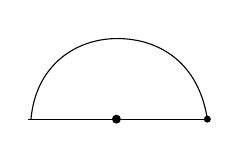
\begin{tikzpicture}[scale=.7]
\draw (-1.7,0) .. controls (-1.6,1.15) and (-.6,1.65) .. (.35,1.4)
.. controls (1.05,1.2) and (1.4,.65) .. (1.5,0);
\draw (-1.75,0)--(1.5,0);
\fill (-.15,0) circle (2.3pt);
\fill (1.5,0) circle (1.8pt);
\end{tikzpicture}}

à deux choses, suivant que $x$ correspond :

\scanpage{57}
% archive foliation: 59
un pt de $K$ d'ordre $\geq2$, ou d'ordre 1 :

\uline{Lemme 2} Soit $K$ un segment topologique $\subset\mathbb C$,
et $x\in K$. \inserted{On suppose $K$ assez régulier (rectifiable suffit ??)} Alors

a) Si $x$ n'est pas extrémité de $K$, alors il existe
\deleted{un voisinage \inserted{ouvert} $U$ de $x$ dans $\mathbb C$, ne contenant pas
d'extrémités de $\unsure{U|K}$, tel que $U\setminus K\cap U$
ait deux composantes connexes $U'$ et $U''$
avec $\overline{U'}\cap U=U'\cup(K\cap U)$, $\overline{U''}\cap U=U''\cup(K\cap U)$, et
\unsure{fonction holo}}

\figure{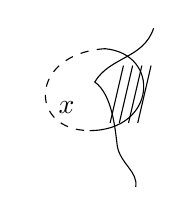
\begin{tikzpicture}[scale=.65]
\draw[dashed] (-.1,1.1) .. controls (-1.6,1) and (-1.6,-.5) .. (-.4,-.5);
\draw (-.4,-.5) .. controls (.9,-.5) and (1,1) .. (-.1,1.1);
\draw (.85,1.5) .. controls (.65,.9) and (.0,.95) .. (-.3,.45)
.. controls (.05,.2) and (.1,-.5) .. (.14,-.8)
.. controls (.2,-1.15) and (.55,-1.3) .. (.5,-1.6);
\foreach \x in {0,.18,.36,.54} {\draw (\x,-.35)--({\x+.26},.77);}
\node at (-.85,-.05) {$x$};
\end{tikzpicture}}

\deleted{\unsure{$f$}} une application continue injective
\inserted{de $\deleted{\unsure{\mathbb C}}H\cap\mathbb D^\circ\longrightarrow\mathbb C$},
\deleted{de $H\cap\mathbb D^\circ$ dans $\mathbb C$, hol. dans $H\cap$
$\mathbb D^\circ\subset\mathbb C$, continue}
holomorphe dans \deleted{$\unsure{\mathbb D\setminus H\supset\mathbb R}$}
\inserted{$(\operatorname{Int}H)\cap\mathbb D^\circ$},
\deleted{$=\,]-1,+1[\quad(\unsure{\ne}\ \mathbb D^{++}\amalg \mathbb D^{--})$}
\deleted{(mais pas \unsure{néct}\ dans deux plans $\mathbb R$)}
(mais pas néc \unsure{hol. au vts de}\ \deleted{dans}
$\delta H\cap\mathbb D^\circ=\,]-1,+1[)$ telle que
$f(\delta H\cap\mathbb D^\circ)\subset K$ et
$f(0)=x$. De plus, pour une rive donnée de
$K$ en $x$, OPS que cette rive est celle déterminée
par \inserted{$\operatorname{Im}f=$} $f(H\cap\mathbb D^\circ)$.

b) Si $x$ est extrémité de $K$, alors $\exists$
$f:H\cap\mathbb D^\circ\longrightarrow\mathbb C$, hol. \inserted{\deleted{et topologique}}
dans $(\operatorname{Int}H)\cap\mathbb D^\circ$, \deleted{et}
\deleted{injective dans $\unsure{\mathbb D^\circ}$ telle que
$\unsure{\{f(-t)=f(t)}$ $\unsure{\{\}}$}
\deleted{\unsure{soit en}\ $f$}
\inserted{telle que $f(0)=0$}
\deleted{$\unsure{f\,]-1,0)}$}
\deleted{$f\mid[-1,0]$ et $f\mid[0,1[$ soient injectifs,}

\figure{\begin{tikzpicture}[scale=.65]
\draw (-.08,2.4).. controls (-.6,1.7) and (.15,1.2) ..(-.25,.65)
..controls(-.7,.2)and(-.08,-.1)..(-.22,-.75);
\draw[dashed](-.85,-.7) arc[start angle=145,end angle=35,radius=1];
\draw (-1.05,-1.35) .. controls (-1.25,-2.25) and (.15,-2.8) .. (.7,-1.95);
\draw (.7,-1.95)..controls(1.1,-1.3)and(.9,-.85)..(.65,-.75);
\node at (-.25,-1.35) {$x$};
\end{tikzpicture}}

\scanpage{58}
\mspage{3}
% archive foliation: 60
et telle que

a) $f\mid(\operatorname{Int}H)\cap\mathbb D^\circ$ est injective, son image $\subset\mathbb C\setminus K$

b) $f(0)=x$, \deleted{$\unsure{f(\pm t)=f(t)}$}

c) $f\mid]-1,0]$ et $f\mid[0,1[$ injectives, avec
même image $\subset K$.

\uline{Scholie} Chaque rive de $K$ \deleted{\unsure{est un}}\inserted{munit} $K$ d'une
structure analytique réelle canonique, via
l'inclusion de $K$ dans $\mathbb C$ (ou dans une
surface conforme quelc), mais le passage
de l'une à l'autre se fait par une
application (identique) qui n'est pas un
iso analytique : les propriétés de régularité
(caractère $C^\infty$, ou analytique réel etc)
reflètent sans doute les propriétés de
régularité correspondantes de $K$ dans $\mathbb C$.
(Ceci \inserted{devrait} se \unsure{magnifier|préciser} dans \deleted{\unsure{le th}}\inserted{un} Scholie
plus circonstancié au Théorème suivant).

\textcircled{3} \uline{Recollement}. On doit avoir un
théorème \unsure{dans le} style du

\scanpage{59}
% archive foliation: 61
\uline{Th. 4} Équivalence de catégories entre

a) Cat. des couples $(X,K,S)$ $X$ surface conforme
à bord compacte, $(K,S)$ complexe top. \deleted{\unsure{cpt}}\inserted{cpt} avec
\[
\delta X\subset K\subset X,\qquad K\text{ assez régulier}\quad\text{(rectifiable suffit)}
\]

\margin{\uline{NB} On ne suppose pas les \unsure{compos. conn.}
de $K\setminus S$ des intervalles
(il peut y avoir des cercles).}

b) Cat des systèmes $(\widetilde X,\widetilde S,\sigma)$, où
$\widetilde X$ est une surface conforme à bord \inserted{compacte},
$\widetilde S$ une partie finie de $\delta\widetilde X$, $\sigma$ une
involution de $\operatorname{\text{Déc}}(\delta\widetilde X/\widetilde S)$, $\sigma$ assez
\unsure{régulière|régulier} (rectifiable suffit).

Le foncteur a) $\longrightarrow$ b) résulte du th. $\unsure{3|2}$,
avec un complément qui explicite les
propriétés de régularité de la fonction-recollement
dont il a été question dans
le lemme 2. Pour le foncteur en sens
inverse, il est connu topologiquement, et
comme faisceau structural conforme
(large) sur $X$ \inserted{$=\widetilde X/R$}, on prend les fonctions
continues qui sont conformes dans $X\setminus K\simeq\operatorname{Int}\widetilde X$.

\scanpage{60}
\deleted{\unsure{3}}\mspage{4}
% archive foliation: 62
Le fait que ça donne bien une structure
conforme à bord \deleted{équivalent} (qui automatiquement
redonne naissance \inserted{avec $K$} à la structure conforme
à bord $\widetilde X$ de départ) équivaut aux
\deleted{lemme suivant :}\inserted{deux cas particuliers suivants}

\deleted{\uline{Lemme 3}

a) Soit $\sigma$ un homéomorphisme rectifiable
(ou plus régulier que ça ?) de $[0,1]$ sur
lui-\deleted{\unsure{même}}, avec $\sigma(0)=0,\ \sigma(1)=1$, alors il existe
une \deleted{courbe}\inserted{\unsure{variété fermée}} $K\subset H\cap\mathbb D^\circ$,
\deleted{\unsure{bien orientée}}\inserted{avec $K\cap\delta H=\{0\}$}
\deleted{, telle que $K\setminus\{0\}$ soit contenu}
$K$ est un intervalle demi-
\deleted{dans $\operatorname{Int}H$}
ouvert d'extrémité 0 ; qui
partage $H\cap\mathbb D^\circ$ en deux comp.
\uline{connexes} $U',U''$. De plus, on trouve un

\figure{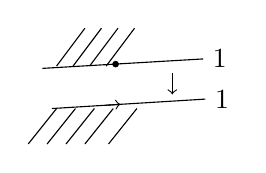
\begin{tikzpicture}[scale=.6]
\draw (-2,1.2)--(1.4,1.4);\node[right] at (1.4,1.4){$1$};
\fill(-.45,1.29)circle(2pt);
\foreach \x in {-1.7,-1.35,-1,-.65}{\draw(\x,1.25)--({\x+.6},2.05);}
\draw[->](.75,1.1)--(.75,.65);
\draw(-1.8,.35)--(1.45,.55);\node[right]at(1.45,.55){$1$};
\draw[->](-.65,.42)--(-.35,.44);
\foreach \x in {-1.7,-1.3,-.9,-.5,0}{\draw(\x,.35)--({\x-.6},-.4);}
\end{tikzpicture}}

\figure{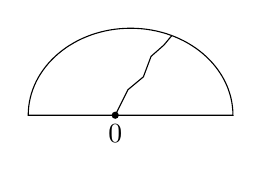
\begin{tikzpicture}[scale=.65]
\draw(-2,0)arc[start angle=180,end angle=0,x radius=2,y radius=1.7]--cycle;
\draw(-.3,0)--(-.05,.5)--(.25,.75)--(.4,1.15)--(.65,1.37)--(.8,1.55);
\fill(-.3,0)circle(2pt);\node[below]at(-.3,0){$\unsure{0}$};
\end{tikzpicture}}
}

\uline{Lemme 3} Cas particuliers

a) Recollement de $H$ à $H$ \inserted{(\uline{deux exemplaires})} suivant un
iso. rectifiable $[0,1]\unsure{\mathrel{\overset{\sigma}{-}}|\xrightarrow{\sigma}}[0,1]$, regardé au
voisinage de 0 [ou variante (\unsure{pour}\ \deleted{\unsure{des}} établir
th. 3) : suivant un isom rectifiable $[-1,1]\xrightarrow{\sigma}[-1,1]$,
regardé au voisinage de 0].

\scanpage{61}
\deleted{\unsure{4}}
% archive foliation: 63
b) Recollement de $\overline H$ à lui $=$ suivant
un isom. rectifiable $[0,1]\xrightarrow{\sigma}[-1,0]$ \inserted{$(\sigma(0)=0)$},
regardé au voisinage du pt 0.

\margin{\uline{12.1}\quad\deleted{\unsure{a)}} c) Soit $C$ une
courbe rectifiable dans \deleted{\unsure{un voisinage de}}\inserted{un ouvert} $U$,
\deleted{\unsure{image de}} $\unsure{\mathbb C}$,
toute \deleted{\unsure{application}} fonction \inserted{complexe}
continue sur $U$ qui est
\unsure{continue|analytique} dans $U\setminus C$, \unsure{est en}
fait holomorphe dans $U$.}

\textcircled{4} \uline{Recollements \deleted{bord à bord}\inserted{des disques}}.
\margin{Le recollement ``bord à bord''}
Cela correspond,
dans le th. 4, au cas où $K$ est une
variété \inserted{(compacte)} de dim 1, $S=\varnothing$. \deleted{Il} Pour avoir
``des \unsure{esp.} de modules'', il est naturel
de dégager des conditions restrictives
naturelles sur l'involution $\sigma$ de
$\delta\widetilde X$.

Pour ceci, \deleted{\unsure{rapp}} on se rappelle que
pour une surface conforme à bord $X$
\inserted{(au lieu de $\widetilde X$)}, et une comp. connexe du bord, soit $C$,
il revient au $=$ de se donner une
structure de droite projective \inserted{rectifiable} sur $C$,
ou un ``bouchage de trou'' en $C$
par un disque \inserted{de bord $C$}, les propriétés de régularité
(\unsure{p.r. à} la structure analytique réelle de $C$)
de la structure de droite projective, reflétant

\scanpage{62}
\mspage{5}
% archive foliation: 64
les propriétés de régularité de $C$ en tant que
cercle \inserted{``intérieur''} dans la surface \deleted{sans bord}\inserted{conforme} $X'$ déduite
par bouchage du trou. D'autre part,
le choix d'un point de $D\setminus C$ équivaut
à celui d'une structure torique
sur $C$ compatible avec la structure de
droite projective réelle (i.e. une réduction
du groupe structural \inserted{$(\unsure{\operatorname{GP}(1,\mathbb R)}\simeq)$}
$\operatorname{GL}(2,\mathbb R)/\mathbb R^*$
au sous-groupe cpt maximal $\operatorname O(2)/\pm1$)
--- et cela équivaut aussi à la donnée
d'une structure \unsure{torique|conique} de $D$ sur \inserted{le bord}
$\delta D=C$. Notons que l'on aura alors une
inclusion canonique
\[
D\subset T_{X',a}
\]
où $a$ est le centre choisi de $D$. On
va expliciter \deleted{ainsi} ces diverses
relations ainsi

\uline{Prop.} Équivalence entre \deleted{la cat. des
surfaces conf.}

\scanpage{63}
% archive foliation: 65
a) Cat. des surfaces conformes à bord $X$,
avec comp. connexe \inserted{compacte} choisie $C$ du bord,
et une structure toroïdale dessus
rectifiable (?) pour la structure
analytique réelle, et

b) Cat. des surfaces conformes à
bord \inserted{$X'$}, avec \deleted{\unsure{le|un}} disque pointé $(D,a)$, $D$
$\subset\operatorname{Int}(X')$ marqué, tel que $\delta D$ soit rectifiable
dans $X'$ (i.e. l'application $\delta D\longrightarrow X'$
rectifiable, pour la structure analytique
naturelle de $\delta D$ comme bord de $D$).

De plus, Pour $(X',a)$ fixé, chaque
disque $D$ autour de $x$ définit un
``disque \deleted{canonique}\inserted{euclidien}'' dans $T_{X',a}$ (au sens de
la structure \inserted{vectorielle} conforme \inserted{(de $T_{X',a}$)}). Comme
\unsure{les|ces} disques forment un torseur sous
$\mathbb R^{*+}$ (par homothéties), \unsure{donc un espace}
de dim $1$, il est clair que l'application

\scanpage{64}
\mspage{6}
% archive foliation: 66
\[
D\longrightarrow o(D)\qquad (\text{``ombre de $D$''})
\]
qui associe à tt disque conforme \unsure{autour de}
$D$ son ombre dans $T_{X',a}$, n'a rien d'injec-
tif. Les \uline{disques ``concentriques''} à $D$
donnent les $\lambda o(D)$ $(0<\lambda\leq1)$, plus
précisément, $D\unsure{\longrightarrow|-}o(D)$ est compatible aux
homothéties de rapport \deleted{$\lambda>0$} $\lambda\in]0,1]$.

Je m'intéresse en fait au cas
où $X'$ est compacte, et munie d'une
\deleted{\unsure{famille}} partie finie de ``pts marqués'', soit
\deleted{$\unsure{I}$}\inserted{$(a_i)_{i\in I}$}, et où on prend une famille
de disques $D_i$ $(i\in I)$ \inserted{\uline{mutuellement disjoints}} autour des $a_i$,
donnant des ombres
\[
o(D_i)\subset T_{X',a_i}.
\]
On cherche des conditions particulières
\inserted{plausibles} sur le système des $D_i$, impliquant
(qui sait ?) qu'il est déterminé par
le système des ombres.

\scanpage{65}
% archive foliation: 67
[On laisse tomber dorénavant les $'$ des $X'$ !]

\deleted{Mais sur $X^*=X\setminus\bigcup D_i$ (si \unsure{chaque composante}
\unsure{connexe} \unsure{$X$ est}}

OPS. $X$ connexe, $I$ non vide --- alors
il y a sur $X^*=X\setminus\bigcup_i D_i^\circ$ (surface
conforme à bord obtenue dans la
découpe de $X$ suivant $\bigcup\delta D_i$) une
\deleted{\unsure{mét}} métrique \deleted{hyperbolique} canonique modulo
constante (qu'on peut d'ailleurs normaliser
par la condition que le volume soit $1$)
\deleted{\unsure{sauf dim $=$}}\inserted{et} canonique \inserted{sans cte} dans le cas
hyperbolique (i.e. quand on n'a
\[
g=0\qquad \underset{\substack{\Vert\\\text{card }I}}{\nu}\in\{1,2\}
\]
) --- dans le cas
\margin{il y a aussi le cas \deleted{\unsure{dans}} \unsure{orienté}
du plan projectif réel $(\simeq S^2/\pm1)$
\deleted{\unsure{privé} d'un disque}\inserted{``avec un trou''}}
hyperbolique le bord est géodésique,
donc dans tous cas le bord est muni
d'une structure torique canonique
provenant de la structure riemannienne.
Il est tentant de restreindre le \inserted{syst. des}
disques envisagés, en exigeant que
les deux structures toriques sur
chaque $\delta D_i$ (provenant soit de $D_i$, soit de $X^*$)

\scanpage{66}
\mspage{7}
% archive foliation: 68
coïncident. Cela signifie donc que
$X$ est déduit de $X^*$ par ``bouchage
de trous \unsure{par disques} canoniques'' (utilisant
les structures toriques sur les
comp. conn. de $\delta X^*$). \deleted{La question}\inserted{Disons alors}
qu'un système de disques $(D_i)_{i\in I}$ dans $X$
\deleted{\unsure{qui n}} autour des $a_i$ est ``admissible''.

\uline{\unsure{Questions|Question :}} Comment cette condition
d'admissibilité se reflète-t-elle en
termes de la géométrie interne de $X$ ?
Par exemple, \deleted{quand} quand $X$ est muni
d'une métrique de \unsure{Bergmann|Bergman} canonique
(cas où $X\not\simeq\mathbb P^1_{\mathbb C}$), quelle est la
relation de cette condition avec celle
que les \deleted{$\unsure{\delta}$}$D_i$ soient des ``disques
géodésiques'' (\inserted{définis} par la condition que
\[
\operatorname{\text{dist. géod}}(x,a_i)\leq r_i
\]
) ?

\margin{supposons hyperbolique i.e. $(g,\nu)\neq(0,1),(0,2)$}
Fixons une \deleted{$X_0$} surface top. \inserted{orientée}
à bord de référence $X_0$, de type $g,\nu$

\scanpage{67}
% archive foliation: 69
et considérons ``l'espace de
Teichmüller à bord'' correspondant
\deleted{$\unsure{T_{g\nu}}$} $TB_{g\nu}$, qui est \deleted{isom.}\inserted{homéo.} à $\mathbb R^{6g-6+3\nu}$
ou mieux, à $\mathbb C^{3g-3+\nu}\times\mathbb R^\nu$. On a une
application
\diagram{\begin{tikzcd}[ampersand replacement=\&]
\underset{\simeq\mathbb C^{3g-3+\nu}\times\mathbb R^\nu}{TB_{g,\nu}} \arrow[r] \&
\underset{\mathbb C^{3g-3+\nu}\deleted{\times\mathbb R^\nu}}{T_{g\nu}}
\end{tikzcd}}
de bouchage des trous, je présume
qu'elle est fibrante \unsure{de faç.},
plus précise, que \deleted{\unsure{dans}\ \unsure{la}}\inserted{c'est la projection}
canonique. \deleted{de} En effet, cela doit
provenir du fait que pour une
sphère à bord \inserted{\unsure{déformante|déformable}} de type $(0,3)$, \deleted{dont}
quand le modèle combinatoire
(\unsure{triangle conducteur}) est fixé, et
qu'on varie seulement \deleted{les} un, deux
ou trois des paramètres ``longueurs''
correspondant aux trois trous, la
sphère ``à bord et ponctuée'' (mono, bi ou
triponctuée suivant les cas) \deleted{\unsure{et le}}\inserted{\unsure{associée|acquise}}

\scanpage{68}
\mspage{8}
% archive foliation: 70
par bouchage des trous correspondants reste
la $=$ (à isom. can. près). Il faudrait,
pour le voir clairement, voir la
relation entre la sphère \inserted{\unsure{bd}} $S(I)$ triponctuée,
associée à la sphère à bord $\Sigma^*$, et ses
paramètres $\ell_i$ $(i\in I)$ comme \unsure{déduite}
\deleted{(\unsure{obtenue}}
de $S(I)$ en enlevant des disques \deleted{que}
$\unsure{D}(\ell_i)$ \inserted{de centre $s_i$ ?}\deleted{qui} dont chacun ne dépend que
des $\ell_i$ correspondants, pas des autres
$\ell_j$.
\margin{?}

Ce point étant supposé acquis, ou quelque
variante, il semble donc bien que
\inserted{(du moins dans le cas hyperbolique orienté)}
pour une surface conforme ponctuée
donnée, \inserted{de type $(g,\nu)$} les familles \inserted{\unsure{admiss.} $(D_i)$} des disques autour
des $a_i$ forment un espace homéom.
à $\mathbb R^\nu$ (où $\nu=\operatorname{card} I$), i.e. à celui
des systèmes d'ombres possibles ! Il
est donc très tentant de faire la

\uline{Conjecture} Pour tt \unsure{surface} conforme
ponctuée (ou \deleted{tout} au moins dans le cas
hyperbolique), l'application \deleted{que}
\[
(D_i)\longmapsto(o(D_i))
\]

\scanpage{69}
% archive foliation: 71
des syst. admissibles de disques \inserted{conformes} autour
des $a_i$, vers l'ens des syst.
de disques \deleted{conformes}\inserted{\unsure{standards|euclidiens}} dans les $T_{X,a_i}$,
est bijective. \deleted{Au niveau des
esp.}

Au niveau des espaces
modulaires de type Teichmüller,
cela donnerait donc une \deleted{\unsure{à}} structure
de fibré principal de groupe
\deleted{\diagram{\begin{tikzcd}[ampersand replacement=\&]TB_{g,\unsure{I|\nu}}\arrow[r,"\sim"]\&T_{g\nu}\end{tikzcd}}}
structural $(\mathbb R^{*+})^I$ : $TB_{g,I}$
sur $T_{g,I}$ $(\operatorname{card}I=\nu)$, \deleted{\unsure{--}}

Si \unsure{la relation} qui précédait
\deleted{(en passant aux log}
\deleted{longueurs} était vraie, cela signifierait
qu'on aurait une section canonique
de ce fibré, ce qui implique
aussi que pour un pt de $T\deleted{B}_{g,I}$,
i.e. une surface bd \inserted{ponctuée} ($\unsure{X_0}$-rigidifiée)
de type $(g,\nu)$, il y aurait un syst.
d'ombres can. dans les $T_{X,a_i}$, i.e. des

\scanpage{70}
\mspage{9}
% archive foliation: 72
métriques euclidiennes \uline{canoniques} sur
les $T_{X,a_i}$, \unsure{décrivant|dérivant} leur structure
conforme. Dans le cas $g\geq2$ et $=$
encore pour $g=1$, cela ne semble pas
inquiétant, puisqu'on a une
métrique canonique sur $X$. Par
contre dans le cas $g=0$, cela semble
étrange, puisque dans ce cas on n'a
\uline{pas} de métrique canonique sur $X$.

\uline{12.1.}

5. \uline{Retour sur le principe de chirurgie conforme}

La formulation des lemmes \inserted{locaux} $2$ et $3$, qui
sont l'ingrédient technique essentiel pour le
th. $4$ (et lui sont équivalents), est un peu
alambiquée. Il est plus élégant de se
réduire à des lemmes globaux du type
uniformisation par le disque $\mathbb D$. Cela
donne le

\scanpage{71}
% archive foliation: 73
\uline{Lemme $4$}
\margin{\uline{NB} il y a une version plus faible de A),
où $\dot U=C$ (sans $I$), \unsure{mais la formulation ci-contre implique A)}}

A) Soit $U$ une partie ouverte bornée
de $\mathbb C$, dont la frontière est \deleted{une}\inserted{réunion de}
courbe de Jordan \deleted{rectifiable. Alors}
$C$, et d'un intervalle \deleted{topologique}
\deleted{il existe une fonction, à savoir}
topologique $\overline I$ tel que
\deleted{$f:\mathbb D\longrightarrow$}
$I\cap C=\{b\}$, \deleted{et} (alors $I\setminus\{b\}$ est
contenu dans la comp. connexe
bornée $V$ de $\mathbb C\setminus C$, et $b$
est une extrémité de $\overline I$,)
\inserted{(alors $U=V\setminus I'$, où $I'=\overline I\setminus\{b\}$)}.
On suppose de plus que $C$ et $I$ soient rectifiables.
Soit $a$ l'autre extrémité de $\overline I$. Alors il
existe une fonction \deleted{continue} $f:\mathbb D\longrightarrow\mathbb C$
telle que

\figure{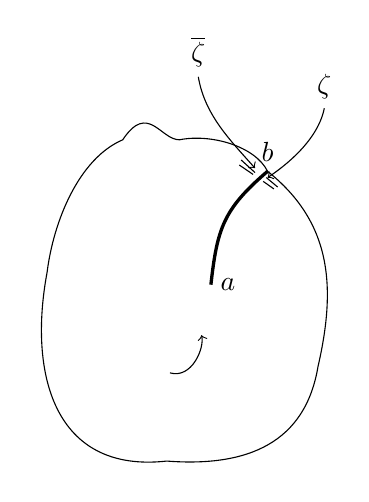
\begin{tikzpicture}[x=.8cm,y=.8cm]
\draw (0,0) .. controls (-1.8,-.2) and (-2.2,1.4) .. (-1.9,3)
 .. controls (-1.8,3.8) and (-1.4,4.8) .. (-.7,5.1)
 .. controls (-.3,5.7) and (-.1,5.1) .. (.2,5.1)
 .. controls (.7,5.2) and (1.4,5) .. (1.6,4.6)
 .. controls (2.6,3.8) and (2.7,2.8) .. (2.4,1.5)
 .. controls (2.2,.3) and (1.3,-.1) .. (0,0);
\draw[very thick] (.7,2.8) .. controls (.8,3.7) and (.9,4) .. (1.6,4.6);
\node[right] at (.7,2.8) {$a$}; \node[above] at (1.6,4.6) {$b$};
\draw[->] (.05,1.4) .. controls (.4,1.3) and (.6,1.8) .. (.55,2);
\draw[->] (.5,6.1) .. controls (.6,5.5) and (1,5.1) .. (1.4,4.65);
\node[above] at (.5,6.1) {$\unsure{\overline\zeta}$};
\draw[->] (2.5,5.6) .. controls (2.4,5.1) and (1.9,4.7) .. (1.6,4.5);
\node[above] at (2.5,5.6) {$\zeta$};
\draw (1.15,4.7)--(1.37,4.55) (1.18,4.78)--(1.4,4.58)
 (1.53,4.44)--(1.7,4.32) (1.58,4.5)--(1.76,4.35);
\end{tikzpicture}}

a) $f$ est continue, et induit une \deleted{\unsure{ho}} bijection
(voire un homéo !) $\mathbb D^\circ\overset\sim\longrightarrow U$.

b) $f(\zeta)=f(\overline\zeta)=b$, et $f$ induit une bijection,
(voire un homéo) $\deleted{\alpha}\inserted{\alpha\setminus\{\zeta,\overline\zeta\}}\overset\sim\longrightarrow C\setminus\{b\}$.
(NB $\zeta=\exp\frac{2i\pi}{3}$, et $\alpha,\beta,\overline\beta$ sont les trois
arcs de $\delta \mathbb D$ déterminés par $1,\zeta,\overline\zeta$).

\figure{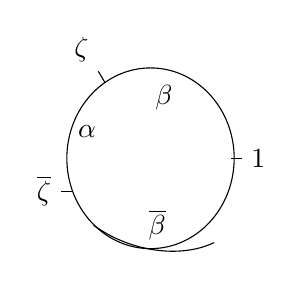
\begin{tikzpicture}[scale=.85]
\draw (0,0) ellipse (1.25 and 1.35);
\draw (1.2,0)--(1.36,0) node[right] {$1$};
\draw (-.68,1.13)--(-.78,1.3) node[above left] {$\zeta$};
\draw (-1.16,-.49)--(-1.34,-.49) node[left] {$\overline\zeta$};
\node at (-.95,.4) {$\alpha$};\node at (.2,.9) {$\beta$};
\node at (.1,-1) {$\overline\beta$};
\draw (-.85,-1) .. controls (-.3,-1.4) and (.45,-1.5) .. (.95,-1.26);
\end{tikzpicture}}

3) $f|\beta$ et $f|\overline\beta$ induisent des bijections de
$\beta$ et $\overline\beta$ sur $\overline I$).
NB a) b) c) peuvent
s'exprimer en disant que $f$ induit un
\deleted{isom}\inserted{\unsure{homéo}} de $\mathbb D$ sur la découpe de $\overline U=\overline V$
suivant $\overline I$ (on scinde $I\cup C=\dot U$).

4) $f|\mathbb D^\circ$ est holomorphe.

\scanpage{72}
\mspage{10}
% archive foliation: 74
\uline{NB 1} Cette fonction est unique, \unsure{dû au fait}
que le groupe des automorphismes \deleted{conformes}
holomorphes de $\mathbb D$ agit de façon simple-
ment transitive sur l'ens des
triples \deleted{\unsure{ordonnés}} de pts distincts $(r,s,t)$ \inserted{sur $S^1=\delta\mathbb D$} qui se
suivent pour l'orientation canonique de
\deleted{$\unsure{\delta\mathbb D}$} $S^1$. \deleted{\unsure{Donc $f$}}

\uline{NB 2} La condition 3) implique qu'on a un
\unsure{homéo} canonique
\[
\varphi:\beta=\widehat{(1,\zeta)}\overset\sim\longrightarrow
\overline\beta=\widehat{(1,\overline\zeta)}
\]
tel que $\varphi(1)=1$, $\varphi(\zeta)=\overline\zeta$).

B) Cette application $\varphi$ est rectifiable. Inverse-
ment, tout \deleted{application}\inserted{homéom} rectifiable $\varphi:\beta\overset\sim\longrightarrow\overline\beta$
provient d'une situation comme en A.
De façon plus précise, \deleted{on peut}\deleted{il existe} (quitte
à \unsure{remplacer} $\overline V$ par $\mathbb D$ par le th. d'uniformi-
sation A) simplifié sans segment intérieur $\overline I$,
et normaliser la situation en \deleted{\unsure{faisant}} envoyant
$a$ en $0$, $b$ en $1$) \deleted{il existe un} Il existe
une application continue
\[
f=f_\varphi:\mathbb D\longrightarrow\mathbb D
\]
telle que

1) $f|\mathbb D^\circ$ soit \deleted{holo} injection holomorphe

\scanpage{73}
% archive foliation: 75
(soit $U=f(\mathbb D^\circ)$)

\figure{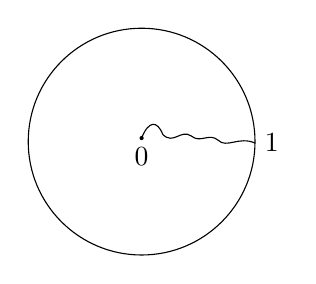
\begin{tikzpicture}[scale=.9]
\draw (0,0) circle (1.6);
\draw (0,.05) .. controls (.1,.3) and (.22,.3) .. (.3,.1)
 .. controls (.45,-.05) and (.55,.18) .. (.7,.08)
 .. controls (.83,-.03) and (.95,.13) .. (1.08,.02)
 .. controls (1.2,-.1) and (1.37,.08) .. (1.6,-.02);
\fill (0,.05) circle (.03);\node[below] at (0,.05) {$0$};
\node[right] at (1.6,-.02) {$1$};
\end{tikzpicture}}

2) $f(\unsure{\omega|0})=0$, $f(\zeta)=f(\overline\zeta)=1$

\deleted{\unsure{3)} $f|\beta$ est un}
$f|(\alpha\setminus\{\zeta,\overline\zeta\})$ \deleted{est}\inserted{induit} un
homéom avec $\delta\mathbb D\setminus\{1\}$

3) \deleted{$\unsure{f(\beta)=I}$} $f|\beta$ et $f|\overline\beta$ sont bijections et
ont $=$ image $\overline I$, \deleted{\unsure{qui est} et $\overline I\setminus\{1\}$}\inserted{contenant $\{1\}$} d'après
2), et $\overline I\setminus\{1\}$ est contenu dans $\mathbb D^\circ$.

4) Soient $f_1:\beta\overset\sim\longrightarrow\overline I$, $f_2:\overline\beta\overset\sim\longrightarrow\overline I$ induites par $f$,
alors $\varphi=f_2^{-1}f_1$

\uline{NB} De nouveau, $f$ est unique. On peut
résumer ce théorème d'uniformisation
au bord dans le \deleted{Scholie}

\uline{Scholie} Il y a corr. $1$-$1$ entre les
données suivantes :

a) Les homéom rectifiables \deleted{\unsure{en}}
\[
\psi:[0,1]\overset\sim-\,[0,1]
\qquad\text{avec }\psi(0)=0\quad(\text{donc }\psi(1)=1)
\]

b) Les segments topologiques \uline{rectifiables}
$\overline I$ dans $\mathbb D$, tels que
\deleted{$\overline I\cap\delta\mathbb D$ soit réduit}
\inserted{$\overline I$ admette $0,1$ comme}
extrémités et \deleted{$\unsure{\overline I\setminus\{1\}\subset\mathbb D}$}
$\overline I\cap\delta\mathbb D=\{1\}$ (i.e.
\deleted{à une extrémité de $\overline I$}
$\overline I\setminus\{1\}\subset\mathbb D^\circ$)

c) Les \deleted{\unsure{a}} applications continues $f:\mathbb D\longrightarrow\mathbb D$
qui ont les propriétés 1) 2) 3) de B) ci-dessus

\scanpage{74}
\mspage{11}
% archive foliation: 76
d) Les séries convergentes
\[
f=\sum_{i\geq0}a_i z^i\qquad(a_i\in\mathbb C)
\]
de rayon de convergence $\geq1$ (donc
définissant $\mathbb D^\circ\longrightarrow\mathbb C$)
\inserted{avec $|f(z)|\leq1$ si $z\in\mathbb D$}, telles que la $f$
se prolonge par continuité en une
fonction $\mathbb D\longrightarrow\mathbb D$, celle-ci ayant les
propriétés 1) 2) 3) de B) ci-dessus.

\textcircled{6}
\margin{\uline{13.1.}}
Soit $(X,C)$ un objet du groupoïde
de Teichmüller analytique complexe
à bord, avec la condition différentiable.
Pour fixer les idées, supposons $X$ connexe,
de type $g,\nu$. Considérons la découpe \inserted{$X'$}
de $X$ suivant $C$, bouchons ses trous
\inserted{(canoniquement en utilisant la structure torique de $\delta X'$)*},
\margin{* via la métrique riemannienne can. de $X'$}
d'où \unsure{surfaces} holomorphes compactes \inserted{sans bord $X''$}, à disques
\inserted{ponctués} marqués, avec des \deleted{iso}\inserted{\unsure{antiiso|antiso}} de \deleted{ces}\inserted{certains de ces} disques
(qui se groupent \deleted{deux à deux} par paires, à l'exception
des $\nu$ disques correspondant à $\delta X$).
On peut considérer $X''$ comme la
normalisée d'une courbe \deleted{$\unsure{R}$}\inserted{$\mathbb C$-alg $X'''$} stable
(au sens de Mumford-Deligne), en

\scanpage{75}
% archive foliation: 77
identifiant les pts des centres des disques
qui se correspondent, et en ponctuant
par les centres des autres disques.
De plus, on obtient, \deleted{avec} pour chaque
point singulier $x$ de $X'''$, correspondant
à une paire $\{x_1,x_2\}$ de points de
$X''$ (centres des deux disques associés),
grâce à l'antiisomorphisme de ces
disques pointés, un élément \deleted{de}\inserted{non nul (i.e. une base)}
de
\[
T_{X'',x_1}\otimes_{\mathbb C}T_{X'',x_2}
\]
i.e. un élément de
\[
T^*_{X'',x_1}\wedge_{\mathbb C^*}T^*_{X'',x_2}.
\]

On trouve ainsi un foncteur de

a) catégorie \inserted{(groupoïde)} des courbes hol. cptes à bord \inserted{$X$} de
type $g,\nu$, avec découpage holomorphe
(avec comme flèches les iso)

vers

b) Catégorie des courbes \inserted{$\mathbb C$-alg} stables de type $(g,\nu)$
$X'''$, munies \inserted{1°)} d'une ``structure de propagation
\unsure{unnodale|nodale}'' en ses pts singuliers, et 2°) d'un
\deleted{structure de \unsure{parallélismes}}\inserted{syst.} admissible de
disques autour des pts marqués.

\scanpage{76}
\mspage{12}
% archive foliation: 78
Au niveau des multiplicités modulaires \inserted{(analytiques réelles.)}
on trouve sûrement un morphisme \inserted{\unsure{pour celles-ci|entre celles-ci}}
\deleted{$\unsure{MB_{g,\nu}}$}
\diagram{\begin{tikzcd}[ampersand replacement=\&]
MDB_{g,\nu} \arrow[r] \& M_{\mathrm{st}}N\deleted{\unsure{{}_{g,\nu}}}D\deleted{\unsure{{}_{g}}}{}_{g,\nu}
\end{tikzcd}}
où $MDB_{g,\nu}$ désigne la multiplicité modulaire
(M) pour les surfaces holomorphes compactes
``découpées'' (D) à bord (B) de type $g,\nu$, et
$M_{\mathrm{st}}ND_{g,\nu}$, celle pour les courbes algébriques
stables (de type loc. constant) \inserted{de type $g,\nu$} à structure de
propagation \unsure{unnodale|nodale} (N) et à système \inserted{adm.} de
disques (D) autour des pts marqués.

Cette flèche est compatible avec les
flèches canoniques vers la cat. des
types combinatoires\inserted{-toriques} de tels objets
(diagrammes MD (Mumford-Deligne en
``\unsure{modulaire|modulaires}'') (\deleted{\unsure{avec poids}}\inserted{incluant} une pondération
des sommets) à structures toriques
associées aux arêtes \ldots\ donnant lieu à un
diagramme commutatif

\scanpage{77}
% archive foliation: 79
\diagram{\begin{tikzcd}[ampersand replacement=\&,column sep=small,row sep=large]
MDB_{g,\nu} \arrow[rr,dash] \arrow[dr] \&\& M_{\mathrm{st}}ND_{g,\nu} \arrow[dl] \\
\& mdt_{g,\nu} \&
\end{tikzcd}}
(dans $mdt$, la lettre $t$ rappelle qu'on a inclus
des structures toriques dans le type
combinatoire). Sûrement aussi, si on
\deleted{définit}\inserted{considère} $MD_{g,\nu}$ (sans bord, ou à bord
``généralisé'' réduit à un ens de $\nu$ pts)
et $M_{\mathrm{st}}N\deleted{D}_{g,\nu}$ (sans structure \inserted{multi}disque) on
aura
\diagram{\begin{tikzcd}[ampersand replacement=\&,column sep=small,row sep=large]
MD_{g,\nu} \arrow[rr] \arrow[dr] \&\& M_{\mathrm{st}}N_{g,\nu} \arrow[dl] \\
\& md_{g,\nu} \&
\end{tikzcd}}
cette fois un morphisme de \deleted{\unsure{de}}
multiplicités \deleted{\unsure{analyti.}} $\mathbb C$-algébriques.
Dans le cas 1), les dimensions \inserted{(réelles)} de
part et d'autre sont celles de $\mathbb C^{3g-3+\nu}\times\mathbb R^\nu$,
dans le cas 2), \inserted{les dim. complexes sont} celle de $\mathbb C^{3g-3+\nu}$.

\scanpage{78}
\mspage{13}
% archive foliation: 80
\uline{Question} Ces flèches sont elles des iso
--- et si oui, comment expliciter un
iso en sens inverse ? \deleted{\unsure{Si}}

Si la détermination conjecturale des
syst. admissibles de disques sur une
surface holomorphe \inserted{compacte} ponctuée (de type
hyperbolique) était connue, on trouve-
rait aisément \deleted{\unsure{des flèches}} un sens
inverse; Au niveau plus naïf des
foncteurs (entre les catégories-solutions
de ces multiplicités) on \unsure{donnerait|fournirait}
ceci : à l'aide d'un \deleted{\unsure{u}}
\[
u_i\in T_{x_i'}^*\wedge_{\mathbb C^*}T_{\unsure{a|x}_i''}^*
\]
\margin{ou ce qui revient au $=$, un
$v_i\,(=u_i^{-1})\in T_{x_i'}^{\vee *}\wedge T_{x_i''}^{\vee *}$}
\deleted{choisissant}\inserted{i.e. un} \deleted{iso} accouplement \unsure{dualisant}
\diagram{\begin{tikzcd}[ampersand replacement=\&]
\deleted{T_{a_i'}^\vee} \arrow[r,draw=none,"{\deleted{\xrightarrow{\sim}}}" description] \& \deleted{T_{a_i''}} \& T_{x_i'}\otimes T_{x_i''} \arrow[r] \& \mathbb C
\end{tikzcd}}
choisissant un \deleted{\unsure{entier}} disque conforme
$D_i'$ en $T_{a_i'}$, \deleted{\unsure{on en déd.}} d'où disque
conforme plein $D_i''$ dans $T_{a_i''}$, on
trouverait \deleted{des} pour le syst. $(D_i')\ (D_i'')$
des \unsure{réalisations} de ces disques comme

\scanpage{79}
% archive foliation: 81
plongés dans $X''$ normalisé de $X'''$ \deleted{dont}\inserted{duquel} on
part, et \deleted{on} trouve des antiiso entre
leurs bords \deleted{de ces} de $D_i',D_i''$ ---
d'où possibilité de les recoller pour
trouver un $X$ surface holo (à bord,
si on a aussi enlevé des disques ouv.
$\mathring D_\alpha^{\unsure{*}}$ correspondant aux pts marqués $x_\alpha$,
sinon une surface à pts marqués),
découpée par les cercles $\Gamma_i$ qui ne
sont \deleted{pas}\inserted{peut-être pas} \unsure{néc.} géodésiques
($??$ \deleted{\unsure{on a}}\inserted{à}
examiner de plus près) mais définissant
des cercles géodésiques uniques,
par les principes de Thurston.

Il faudrait voir que le résultat
obtenu ne dépend pas du choix des
paires $(D_i',D_i'')$ mut.\textsuperscript{t} polaires, il y
a un argument heuristique pour
cela tout à fait vaseux, consistant
à dire qu'une petite variation de \unsure{celle|cette},

\scanpage{80}
\mspage{14}
% archive foliation: 82
paire ne change rien; car si on remplace
$D_i'$ par $\lambda D_i'$, donc $D_i''$ par $\frac1\lambda D_i''$, avec $\lambda\in\mathbb R^{*+}$
voisin de 1, ces deux relations vaudront
pour les disques obtenus dans \inserted{le normalisé} $X''$
(c'est probablement tout à fait faux !)
et on obtiendrait la $=$ surface recollée $X$
mais les $\Gamma_i$ remplacés par des cercles
``voisins'' $\Gamma_i'$.

Le cas-clef à comprendre sans
doute est celui où $(g,\nu)=(0,4)$,
i.e. le mécanisme du recollement
de deux ``pantalons'' de Thurston,
donc pour \deleted{\unsure{ces cas}}\inserted{deux} ens. $\varepsilon',\varepsilon''$ à deux
éléments, fixes, les foncteurs des
\[
\left\{\begin{gathered}
\text{pantalons de type combinatoire }\varepsilon'\amalg\{s\},\quad\varepsilon''\amalg\{t\},\\
\text{recollés suivant }\{s,t\},\quad\deleted{\text{donné}}\ \text{suivant}\\
\text{les données }(\ell_i)_{i\in\varepsilon'\amalg\varepsilon''\amalg\unsure{u}}
\in(\mathbb R^{*+})^{\varepsilon'\amalg\varepsilon''\amalg\unsure{u}},\\
\text{et }\theta\in\mathbb U_{\varepsilon'\unsure{\wedge|\times}\varepsilon''}\quad\text{qui fixe le recollement}
\end{gathered}\right.
\]
vers

\scanpage{81}
% archive foliation: 83
\[
\left\{\begin{gathered}
\text{paires de pantalons }\deleted{\text{\unsure{dég.}}}\inserted{\text{\unsure{généralisés}}}\inserted{X',X''},\ \inserted{\text{\unsure{à trous}}}\ \text{indexés}\\
\text{par }\varepsilon'\amalg\{s\},\quad\varepsilon''\amalg\{t\},\quad\text{avec }s,t\ \text{correspondant}\\
\text{aux }\deleted{\text{bords}}\ \text{composantes ponctuelles du}\\
\text{bord, avec les paramètres }(\lambda_i)_{i\in\varepsilon'\amalg\varepsilon''}\in\unsure{(\mathbb R^{*+})^{\varepsilon'\amalg\varepsilon''}}\\
\text{et un isom d'identification}\\
\text{des }\mathbb C^*\wedge_{\pm1}(\varepsilon'\wedge\varepsilon'')
\end{gathered}\right.
\]
Une fois ce cas compris, et revenant
alors au cas général, il faudrait déjà,
pour un type de découpage donné
incarné par un diagramme MD
dans $md_{g,\nu}$, comprendre l'application
sur les groupes fondamentaux
induite par
\diagram{\begin{tikzcd}[ampersand replacement=\&]
\unsure{\varphi})\quad MD\deleted{B}_{\unsure{g}} \arrow[r] \& M_{\mathrm{st}}N\deleted{\unsure{D}}_{g,\nu},
\end{tikzcd}}
ceux du deuxième membre étant
essentiellement compris, en termes de
groupes de Teichmüller spéciaux
--- \uline{mais il doit en être pareil pour le
premier} ! Également, il ne devrait
pas être bien dur de vérifier si $\unsure{\varphi}$

\scanpage{82}
\mspage{15}
% archive foliation: 84
est étale, en calculant i.e. interprétant
son application tangente.

\scanpage{84}
% archive foliation: 86
\fbox{\unsure{Modulis|Moduli} $M_{0,4}$ et l'octaèdre}

$I$ ens de card. 4 d'où
\[
J=\unsure{P|\mathcal P}_{2,2}(I),\quad V(J)\ \text{plan vectoriel sur }\mathbb F_2\text{ avec }V(J)^*\simeq J,
\]
$V(J)\subset\unsure{\mathfrak S}_I$ formé de l'identité et des ``bitranspositions''.

On s'intéresse aux droites projectives (sur $\mathbb C$ disons --- \unsure{ça}
marcherait sur tt corps $k$ \inserted{de car. $\ne2$}) munies de $I\hookrightarrow X$.
(plus précisément $I_{\mathbb C}\hookrightarrow X$, ou $I\longrightarrow X(\mathbb C)$ \ldots).
L'opération de $V(\unsure{I|J})$ sur $I$ se prolonge en une opération de
$V(J)$ sur $X$
\[
V(J)\hookrightarrow G_X=\operatorname{Aut}(X)
\]
Soit
\[
\begin{gathered}
S=\text{ens des pts dans }X\text{ qui sont fixes par un}\\
\text{élément de }J=V(J)^*\\
\operatorname{card}S=6
\end{gathered}
\]
\margin{\uline{\unsure{Commençons}} \uline{par \unsure{ça}}}
\figure{\begin{tikzpicture}\draw (0,0)--(0,1.1);\end{tikzpicture}}
En fait, on trouve que \deleted{\unsure{pour les}}\inserted{les} opérations \inserted{fidèles} d'un gr. abstrait $V$
sur un $X$, i.e. les plongements $V(\unsure{J})\hookrightarrow G_X$, sont tous
équivalents (modulo autom. intérieurs de $G_X$)
et sont (pour une base fixée \inserted{$e_0,e_1$}) équivalentes à l'opération sur $\mathbb P^1$
\diagram{\begin{array}{rcll}
u(e_0)&=(z\longmapsto-z)=\begin{pmatrix}-1&0\\0&1\end{pmatrix}& &\text{pts fixes }0,\infty\\[3pt]
u(e_1)&=(z\longmapsto1/z)=\begin{pmatrix}0&1\\1&0\end{pmatrix}& &\text{pts fixes }\pm1\\[3pt]
u(e_0+e_1)&=(z\longmapsto-1/z)=\begin{pmatrix}0&-1\\1&0\end{pmatrix}& &\text{pts fixes }\pm i
\end{array}}
Les \deleted{\unsure{quatre groupes}}\inserted{sous-groupes} isom. à $D_2$ de $G_X$ correspondent 1-1 aux
parties $S$ de cardinal 6 de $X$, isom. à $(\mathbb P_1,\{0,\infty,\pm1,\pm i\})$.
\margin{parties octaédriques d'une droite projective}
Le normalisateur $\Gamma$ d'un tel \deleted{$\unsure{D_2}$} sous-groupe $V$ \inserted{dans $G_X$} est isomorphe
au groupe \deleted{des rotations} $\unsure{\mathfrak S}_4$ (de façon non canonique), plus
précisément, si $V=V(J)$ avec $J=\unsure{P|\mathcal P}(I)$ \inserted{i.e. si $I$ est un $V$-torseur}, on trouve \deleted{des} iso
de suites exactes
\diagram{\begin{tikzcd}[ampersand replacement=\&,column sep=small]
\&\& \deleted{\unsure{\operatorname{Aut}(I)}} \arrow[d,equal] \&\& \\
\unsure{1} \arrow[r] \& V \arrow[r] \arrow[d,equal] \& \unsure{\mathfrak S}_I \arrow[r] \arrow[d] \& \operatorname{Aut}(V) \arrow[r,dash] \arrow[d,equal] \& 1 \\
1 \arrow[r] \& V \arrow[r] \& \Gamma \arrow[r] \& \operatorname{Aut}(V) \arrow[r,dash] \& 1
\end{tikzcd}}
défini modulo autom. intérieurs par un élément de $V$.
Quand $I$ est le torseur trivial, \unsure{se donner|on donne} un tel \deleted{iso}\inserted{iso d'ext.}

\scanpage{85}
% archive foliation: 87
revient à se donner un scindage de l'extension
\diagram{\begin{tikzcd}[ampersand replacement=\&,column sep=small]
(\ast)\qquad 1 \arrow[r] \& V \arrow[r] \& \Gamma \arrow[r,dash] \arrow[d,equal] \& \operatorname{Aut}(V) \arrow[r,dash] \arrow[d,"\simeq",draw=none] \& 1 \\
\&\& \operatorname{Nor}_G(V) \& \unsure{\mathfrak S}_J \&
\end{tikzcd}}
En termes géométriques, ces scindages sont associés
aux quatre systèmes de \inserted{paires de} faces antipodiques sur l'
octaèdre. \deleted{Ainsi, les} L'octaèdre combinatoire (non orienté
a priori) se définit à partir de l'ens $S$ de
ses sommets, et l'antipodisme \deleted{sur} $S$, de la façon
habituelle; ses faces sont les parties à trois éléments \deleted{qui}
$S'$ telles que $S'\cup\uline{a}(S')=S$. Pour un tel triplet,
le sous-groupe de $\Gamma$ qui l'invarie est un scindage
de l'extension $(\ast)$.

Le groupe $\Gamma$ est le groupe des autom. de
$S$ qui conserve \deleted{\unsure{des}} structure octaédrique
\uline{orientée} (définie par l'ens \inserted{$F\subset\unsure{P|\mathcal P}_3(S)$} des \deleted{8} faces \deleted{\unsure{et}} l'ens
des arêtes \inserted{$A\subset\unsure{P|\mathcal P}_2(S)$} est défini comme l'ens des parties de
card 2 contenues dans une face), par le choix
d'une orientation $\omega$. Choisir cette orientation, revient \inserted{donc}
à la choisir dans le cas standard $X=\mathbb P^1$, $S=\{0,\infty,\pm1,\pm i\}$,
où une face est $\{0,1,i\}$, et les faces \inserted{\uline{orientées}} $\overrightarrow{\{0,1,i\}}$ et
$\overrightarrow{\{0,1,-i\}}$ sont \uline{opposées}. Donc le choix d'une orientation
combinatoire revient au choix d'une racine carrée de
$-1$.

Pour un sous-groupe $V\simeq D_2$ de $G_X$, on désigne
par $\operatorname{Oct}(V)\subset X$ l'octaèdre correspondant, par $I(V)=F/\uline{a}_{\unsure{I|F}}$
l'ens de ses paires de faces antipodiques. Mais : $\Gamma(V)=\operatorname{Nor}_G(V)$

\scanpage{86}
% archive foliation: 88
qui opère sur $\operatorname{Oct}(V)$, opère sur $I(V)$, et on trouve
\diagram{\begin{tikzcd}[ampersand replacement=\&]
\Gamma(V) \arrow[r,"\sim"] \arrow[d,equal] \& \unsure{\mathfrak S}_{I(V)},\\
\operatorname{Aut}^+(\operatorname{Oct}(V)) \&
\end{tikzcd}}
et cet iso \deleted{$\unsure{\operatorname{Aut}}$} définit une structure de
$V$-torseur sur $I(V)$. (Ceci résulte de la théorie
combinatoire de l'octaèdre, ou du cube c'est kif kif.)

\uline{Proposition} Soit $X$ droite projective \unsure{réelle} sur un corps alg. clos $k$
(il suffit qu'il \deleted{contienne} soit stable par extraction des racines
carrées) de car. $\ne2$, et $G=\operatorname{Aut}_kX$. Alors il y a corr 1-1
entre

a) les sous-groupes $V$ de $G$ isom. à $D_2$

b) \rule{3cm}{0.2pt} $\Gamma$ de $G$ isom. à $\unsure{\mathfrak S}_4$ \deleted{\unsure{un}}

c) les parties $S\in\unsure{P|\mathcal P}_6(X(k))$ qui sont ``octaédrales'', i.e.
\deleted{\unsure{telles que}}\inserted{isom. à} $(\mathbb P^1_k,\{0,\infty,\pm1,\pm i\})$

par
\[
\begin{aligned}
\Gamma&=\operatorname{Nor}_G(V)\\
V&=\inserted{\text{unique}}\ \text{sous-groupe }\deleted{\text{\unsure{invariant isom. à}}}\inserted{\text{inv. de }\Gamma\ \text{isom. à}}\ D_2\ \deleted{\unsure{\subset G}}\\
S&=\text{ens de ramification de l'action de }V\text{ sur }X
\end{aligned}
\]
\deleted{\unsure{ou de l'action}}
(\uline{NB} $\Gamma$ a un ens de ramification
plus grand qui comprend, en plus de $S$,
les ``milieux d'arêtes'' et ``centres des faces''
de l'octaèdre,

\margin{\uline{Cor} la catégorie (quand $k$ fixé)
des couples $(X,V)$ (ou $(X,\Gamma)$
$(X,S)$) $\unsure{\longrightarrow|\text{est}}$ équivalente à celle
des octaèdres \inserted{\unsure{combin.}} \uline{orientés}, une
fois choisi \deleted{\unsure{a}} une racine
carrée de $-1$ dans $k$. Mieux : la
cat. des couples $(X,V)$ $\unsure{\longrightarrow|\text{est}}$ équivalente
à celle des couples $(\operatorname{Oc},\varphi)$
où $\operatorname{Oc}$ est un octaèdre combinatoire et
$\varphi:\{\pm i\}\overset\sim\longrightarrow\unsure{\operatorname{or}}(\operatorname{Oc})$.}

Dans l'ensemble $S$, on a un antipodisme $\uline{a}_S=\uline{a}_V$
défini par la condition que pour $\sigma\in V^*$, $a_S$ \deleted{est}\inserted{induit} la transposition
de $X^\sigma$ (de cardinal 2). On définit sur $S$ une
structure octaédrale, admettant $\Gamma$ comme groupe des
autom. orientés, et $\uline a$ comme antipodisme, via l'antipodisme
(les faces sont les parties $S'\in\unsure{P|\mathcal P}_3(S)$ telles que $S'\cup-S'=\unsure{S'|S}$).

\scanpage{87}
% archive foliation: 89
\uline{NB} On sait que la donnée d'un octaèdre \inserted{comb.} non orienté
revient à celle d'un système $(I,\omega)$, \deleted{\unsure{dans}} $\operatorname{Ens}_4\times\operatorname{Ens}_2$,
ens des \unsure{octo-quartes} et des orientations. Ici $\omega=\{i,-i\}$, \deleted{\unsure{et on}}
\deleted{par la donnée de $I$, que}\inserted{Mais ici on n'a pas $I$ qui est \unsure{abstrait}, mais}
$S$, qui est un ens de cardinal 6 sur lequel $V$ opère.
La condition à mettre \deleted{est} pour que ceci définisse une
\deleted{des} structure octaédrale (dont $S$ sera l'ens des sommets)
est que $\forall\sigma\in V^*$, \deleted{$\unsure{V}$} $\operatorname{card}S^\sigma=2$, et $S=\bigcup_{\sigma\in V^*}S^\sigma$
(réunion forcément disjointe) (cela entraîne que
$\sigma$ opère sur $(S\setminus S^\sigma)$ par transposition de \deleted{\unsure{les}}\inserted{\unsure{chacune}} des deux
composantes $S^{\sigma'},S^{\sigma''}$, ici $V^*=\{\sigma,\sigma',\sigma''\}$). Donc la
donnée de \deleted{$\unsure{S,V\subset}$} $(V,S,u:V\hookrightarrow\unsure{\mathfrak S}_S)$, ou $(S,V\subset\unsure{\mathfrak S}_S)$,
équivaut à celle de $S$, avec une involution sans pts fixes
$a$ (ayant les $S^\sigma$ comme orbites).

Revenant à la donnée d'un $V$ qui opère \inserted{fid.\textsuperscript{t}} sur $X$,
considérons une orbite \inserted{$I$} de $V$ sur $X^*=X\setminus S(V)$.
Donc $I$ est un torseur sous $V$. La donnée de
$(X,I,I\hookrightarrow X)$ équivaut à celle de $(X,I,V(I)\hookrightarrow G_X,$
$I$ orbite de $V(I)$ dans $X)$, et on se propose de
comparer le $(V=V(I))$-torseur $I$, avec le
$V$-torseur $I(V)$ \inserted{$=I(V,X)$} défini via l'octaèdre $\operatorname{Oc}(V)=\operatorname{Oc}(V,X)$.

En termes de \inserted{$I\deleted{\unsure{V}},\{\pm i\}$}, on peut définir un octaèdre \deleted{\uline{orienté}}
canonique \deleted{\unsure{sans base marquée, défini par la}}
condition que \deleted{\unsure{le groupe de ses} \illegible{1} \unsure{soit} $V$} \inserted{l'ens de ses \unsure{2|8} \unsure{faces} ``\unsure{ant.}'' $I_\pm$, l'ens de ses orientations $\{\pm i\}$}
\deleted{\unsure{bipartitions}}.
Cet \deleted{oct.} octaèdre, \deleted{une fois choisi un $i=\sqrt{\unsure{1|-1}}$,} peut
se réaliser canoniquement \deleted{\unsure{par des cas}}\inserted{comme un} $(X,S)$
$=(X(I),S(I))$. On a un iso can

\scanpage{88}
% archive foliation: 90
\[
X(I)/V(I)\simeq X(J)\qquad\text{où }J=J(I)\text{ comme dessus}
\]
Ceci dit soit \deleted{$I\hookrightarrow X$}\inserted{une opération de $V$ sur $X$}
\deleted{on a donc \unsure{de} $X$ une opération $V=V(I)$}\inserted{$V$}$\hookrightarrow G_X$, d'où un $I(V)$ $V$-torseur
des bifaces de $\operatorname{Oc}(V)$, et on a \deleted{$X\simeq$}
\[
X\simeq X(I(V))\qquad\text{iso. canonique},
\]
(et non $X\simeq X(I)$). Mais pour \deleted{un} deux torseurs
$T,T'$ sous un $=$ $V$, on aura
\[
X(T\wedge T')=X(T)\wedge_V T'
\]
\margin{\figure{\begin{tikzpicture}\draw (0,0)--(0,.65);\end{tikzpicture}} à expliciter}
Soit donc
\[
\begin{gathered}
\uline t=\unsure{\delta|\tau}(I,X)\text{ le }V\text{-torseur tel que}\quad I(V)\simeq I\wedge_V\delta\\
\text{i.e.}\qquad\delta\simeq I(V)\wedge I^{-1}.
\end{gathered}
\]
On aura
\[
\boxed{X=X(I(V))=X(I)\wedge_V\uline t}
\]
\deleted{Donc et l'on} donc
\[
\boxed{X/V\simeq X(I)/V\simeq\unsure{Z|X}(J)}
\]

En résumé :

\figure{\begin{tikzpicture}\draw (0,0)--(0,2);\end{tikzpicture}}
\uline{Cor à Prop} \deleted{La donnée, d'un \unsure{gr.} $V\simeq D_2$}\inserted{Pour $I\in\operatorname{Ob}\operatorname{Ens}_4$}
donné, d'où $J$ et
$V=V(J)$, la donnée d'un $X$ et d'un plongement
$V\hookrightarrow G_X$ équivaut à la donnée d'un torseur $\uline t$ sous $V$,
via
\diagram{\begin{tikzcd}[ampersand replacement=\&]
\delta \arrow[r,mapsto] \& X(I)\wedge_V\deleted{\unsure{\delta}}\uline t
\end{tikzcd}}
On a donc
\[
X/V\simeq\unsure{Z|X}(J)\qquad\text{(iso. canonique)}.
\]

\uline{\unsure{Cor à Cor}}, \inserted{Donc} la donnée de $(X,I\hookrightarrow X)$ équivaut à
celle de a) un pt $\zeta$ de $Z(J)^*$, b) un $V$-torseur $\uline t$,
\deleted{c) un $V$-isom \unsure{un tel} \unsure{point} $X=X(I)\wedge_V\uline t$,}
et
\deleted{$X_\zeta=\text{fibre de}$}
\[
X_\zeta=X(I)_\zeta\wedge\uline t\simeq I\qquad\text{i.e.}\quad\uline t=I\wedge X(I)_\zeta^{-1}.
\]

\scanpage{89}
% archive foliation: 91
\figure{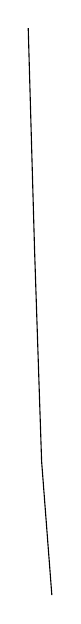
\begin{tikzpicture}\draw (0,0)--(.08,-2.8)--(.17,-5.5)--(.3,-7.2);\end{tikzpicture}}
\uline{Théorème} Soit $k$ un corps alg. clos de car. $\ne2$,
\deleted{Soit $I$ un ens de card $4$, d'où $J$ de card. $3$ et $V=V(J)$. Considérons}

Considérons le groupoïde des $(X,I\hookrightarrow X)$, où $X$ est
une droite projective sur $k$, \deleted{\unsure{tel}}\inserted{$I$ de card $4$}.
Ce groupoïde est équivalent à celui des couples $(I,\zeta\in Z(J(I))^*)$,
en associant à ce couple
\[
X=X(I)\wedge_{\underbrace{V(J(I))}_{\text{ou }V(I)}}t(\zeta,I).
\]
\margin{où $t(\zeta,I)$ est le $V(I)$-torseur $I\wedge X(I)_\zeta^{-1}$}
$I\hookrightarrow X$ est la fibre \inserted{$X_\zeta$} de $X$ en $\zeta$, compte tenu que
\[
\begin{gathered}
X/V(I)\simeq X(I)/V(I)\simeq\unsure{Z|X}(J)\\
X_\zeta\simeq X(I)_\zeta\wedge t(\zeta,I).
\end{gathered}
\]

(\deleted{\unsure{Si}} si $I$ est muni d'un pt $i_0$, on a une description
de $X$ comme $X(I)\wedge_{V(I)}X(I)_\zeta^{-1}$ ; c'est isom. à $X(I)$ une
fois choisi un \unsure{sommet|élément} de $X(I)$ au dessus de $\zeta$.

De façon plus générale, \deleted{\unsure{donc}} la donnée d'un
isom. ``admissible'' $X\simeq X(I)$ équivaut à celle d'un
$V$-isom $I\simeq\deleted{\unsure{Y}}X(I)_\zeta$.

\scanpage{91}
% archive foliation: 93
\margin{\uline{Déc 83}}
\uline{Courbes elliptiques réelles}

Soit $k$ un anneau (pas néc comm.)

\deleted{$M$ un $k$-\unsure{module}}
Considérons la catégorie des $k$-Modules
$M$ munis d'un \unsure{autom.} $\sigma$ \deleted{tel que}
tel que
\[
\begin{array}{ll}
\text{a)}&\sigma^2=\operatorname{id}\\
\text{b)}&2\operatorname{id}_M\text{ injectif (on dit alors }M\text{ 2-régulier)}
\end{array}
\]
A un tel couple $(M,\sigma)$, \inserted{nous} associons le couple
$(P,Q,m)$ de deux \inserted{$k$-}modules pour lesquels $2\operatorname{id}_P$ et $2\operatorname{id}_Q$
sont injectifs (i.e. $P,Q$ 2-réguliers), et
$m\subset P/2P\oplus Q/2Q$ \inserted{sous $k/2k$-module} avec
$m\cap P/2P=0$, $m\cap Q/2Q=0$
(c'est deux sous-modules $p'\subset p\overset{\mathrm{def}}=P/2P$, $q'\subset q=Q/2Q$,
et un iso. $p'\simeq q'$), de la façon suivante
\[
\begin{aligned}
P=M_+&=\operatorname{Ker}(\operatorname{id}_M-\sigma)=\{x\in M\mid\sigma x=x\}\\
Q=M_-&=\operatorname{Ker}(\operatorname{id}_M\unsure{-|+}\sigma)=\{\unsure{x|m}\in M\mid\sigma x=-x\}.
\end{aligned}
\]
NB $M_+\cap M_-=0$ dans $M$, car $M$ 2-régulier, donc
\margin{!}
\[
2M\subset M_+\oplus M_-\subset M\deleted{\subset\tfrac12(M_+\oplus M_-)}
\quad\text{car }\forall x\in M,\text{ on a }2x=\underbrace{(x+\sigma x)}_{M_+}+\underbrace{(x-\sigma x)}_{M_-}.
\]
soit
\diagram{\begin{tikzcd}[ampersand replacement=\&,column sep=small,row sep=small]
M' \arrow[d,equal] \arrow[r,phantom,"\subset"] \& M_+\oplus M_-=P\oplus Q \& \unsure{\sigma}\\
2M \&\&
\end{tikzcd}}
on a donc
\[
\deleted{\unsure{M'\supset}}2P\oplus2Q\subset M'\subset P\oplus Q.
\]
donc $M'$ est l'image d'un sous-module $m$ de
\[
(P\oplus Q)/2P\oplus2Q\simeq\underbrace{P/2P}_p\oplus\underbrace{Q/2Q}_q,
\quad\text{et on vérifie que}
\]
\[
\left\{\begin{aligned}
m\cap\deleted{\unsure{q}}p&=0\quad\text{i.e.}\quad
\underbrace{M'\cap(P+(2P+2Q))}_{M'\cap P+(2P+2Q)}=(2P+2Q)\quad\text{car }M'\cap P=2P\\
m\cap q&=0\quad\text{car}\quad M'\cap Q+(2P+2Q)=\unsure{2Q}\quad\text{car }M'\cap Q=2Q
\end{aligned}\right.
\]
\margin{puisque $2x\in P$ i.e. $2\sigma x=2x$ implique $x\in P$ i.e. $\sigma x=x$}

D'ailleurs \deleted{$\unsure{M'\oplus Q}$} $(M,\sigma)$ se reconstitue à isom can près de
$(P,Q,m)$, car $M'\subset P\oplus Q$ se reconstitue, et
\deleted{\unsure{M}}$\sigma_{M'}$ aussi \unsure{l'étant} par $\operatorname{id}_P\oplus(-\operatorname{id}_Q)$,
Or $2\operatorname{id}_M\deleted{\unsure{M}}:M\longrightarrow M'$ est un iso de $(M,\sigma_M)$ vers $(M',\sigma_{M'})$.

\uline{Prop} Le foncteur précédent $(M,\sigma)\longmapsto(P,Q,m)$ est une équivalence
de catégories.

\uline{Cor} Supposons $k$ \deleted{\unsure{un anneau}\unsure{ intègre}\unsure{ de Dedekind}\unsure{ principal|projectif}}
\inserted{comm.}\inserted{\unsure{et} $k$ 2-régulier}, prenons
\deleted{\unsure{des}}\inserted{$(M,\sigma)$} $M$ \deleted{\unsure{libre|projectif}}\inserted{\unsure{projectif}} de \unsure{rang} $2$
avec $\sigma\ne\operatorname{id}_M,-\operatorname{id}_M$, alors la cat
\deleted{de}\inserted{des} \unsure{formés} \deleted{\unsure{par}\unsure{ ces}\unsure{ objets}\unsure{ est}}\inserted{\unsure{on a} $\sigma^2=\operatorname{id}$}
\unsure{($P,Q$ inv. de rg $1$)}
équivaut à celle des paires $(P,Q)$ avec $P,Q$ inv., et
$p'\subset P/2P$, $q'\subset Q/2Q$ et $p'\overset{u}\simeq q'$ donné.

\scanpage{92}
% archive foliation: 94
\begin{verbatim}
//*   CRAY2   0344        I
        00000000      00000000    555555555555       11
      0000000000    0000000000   555555555555       111
    00      0000  00      0000  55               1111
   00     00 00  00     00 00  55                 11
  00     00 00  00     00 00  55                 11
 00     00 00  00   00   00  555555555           11
00  00    00  00  00    00  555555555           11
00 00     00  00 00    00          55         11
0000      00  0000     00          55        11
000       00  000      00         55        11
0000000000    0000000000   555555555555   1111111111
00000000      00000000    55555555555   1111111111
\end{verbatim}
\[
\deleted{M'}\quad P\oplus Q\supset M'\supset2P\oplus2Q
\]
\deleted{\unsure{de}}
\[
\begin{aligned}
\sigma(x,y)&=x-y\\
(1+\sigma)(x,y)&=2x\\
(1\unsure{-|+}\sigma)(x,y)&=2y
\end{aligned}
\]
\[
\deleted{\unsure{\forall x\in P,\ \exists x,y\in M'},\ (1+\sigma)(x,y)=\unsure{x}\quad\text{i.e. }2x}
\]
\[
P=\qquad\deleted{\unsure{x\in(x,y)\in M'}}\qquad
(\deleted{x,y})x+2y\in M'
\]
\[
\left\{\begin{aligned}M'\cap P&=2P\\M'\cap Q&=2Q\end{aligned}\right.
\qquad\text{i.e.}\quad
\underbrace{M'\cap(P+2Q)}_{(M'\cap P)+2Q}=2P+2Q
\]
\begin{verbatim}
 CCCCCCCCCC   RRRRRRRRRRR    AAAAAAAAAA   YY        YY   2222222222
CCCCCCCCCCCC  RRRRRRRRRRRR  AAAAAAAAAAAA  YY        YY  222222222222
CC        CC  RR        RR  AA        AA   YY      YY   22        22
CC            RR        RR  AA        AA    YY    YY             22
CC            RR        RR  AA        AA     YY  YY              22
CC            RRRRRRRRRRRR  AAAAAAAAAAAA      YYYY               22
CC            RRRRRRRRRRR   AAAAAAAAAAAA       YY               22
CC            RR    RR      AA        AA       YY              22
CC            RR     RR     AA        AA       YY             22
CC        CC  RR      RR    AA        AA       YY            22
CCCCCCCCCCCC  RR       RR   AA        AA       YY           222222222222
 CCCCCCCCCC   RR        RR  AA        AA       YY           222222222222
\end{verbatim}
\[
m\subset\underbrace{P/2P}_p\times\underbrace{Q/2Q}_q
\]
sous-module de $k/2k$ modules
\[
\begin{aligned}m\cap p&=0\\m\cap q&=0\end{aligned}
\qquad
\begin{aligned}m&\longrightarrow p\quad\text{injectif}\\m&\longrightarrow q\quad\text{injectif}\end{aligned}
\]
\begin{verbatim}
****A  START  JOB  344  CRAY2       ROOM     3.08.27 PM 19 AUG 82  R6.PR1  SYS JES2  JOB 344  START  A****
****A  START  JOB  344  CRAY2       ROOM     3.08.27 PM 19 AUG 82  R6.PR1  SYS JES2  JOB 344  START  A****
****A  START  JOB  344  CRAY2       ROOM     3.08.27 PM 19 AUG 82  R6.PR1  SYS JES2  JOB 344  START  A****
****A  START  JOB  344  CRAY2       ROOM     3.08.27 PM 19 AUG 82  R6.PR1  SYS JES2  JOB 344  START  A****
****A  START  JOB  344  CRAY2       ROOM     3.08.27 PM 19 AUG 82  R6.PR1  SYS JES2  JOB 344  START  A****
****A  START  JOB  344  CRAY2       ROOM     3.08.27 PM 19 AUG 82  R6.PR1  SYS JES2  JOB 344  START  A****

DERNIERE MISE A JOUR DE JOURNAL : 11-08-82
ATTENTION .........
   ]         UN ARRET EXCEPTIONNEL POUR PREPARER L'ARRIVEE DE NOUVELLES
   ]         UNITES AURA LIEU DU VENDREDI 20 AOUT A 17H 30 AU LUNDI
   ]         23 AOUT A 8H.
\end{verbatim}
\deleted{
$x\mapsto2x:M\longrightarrow M$ injectif

\deleted{\unsure{k}} $k\longrightarrow k'=k[\frac12]$
\[
M\subset M\otimes k'=M'=M'_+\oplus M'_- =\unsure{M_{+k'}}
\]
\margin{\uline{$M$ plat sur $\deleted{\unsure{k[\frac12]}}k$}\par donc $x\mapsto2x$\par $M\longrightarrow M$\par injectif}
\[
\begin{aligned}
M_+&=\{\unsure{m|x}\in M\mid\sigma x=\unsure{x}\}=\operatorname{Ker}(1-\sigma)\\
M_-&=\{\unsure{m|x}\in M\mid\sigma x=-x\}=\operatorname{Ker}(1+\sigma)
\end{aligned}
\]
\[
M_+\cap M_-=0\qquad M/M_++M_-\text{ annulé par }2
\]
\[
2x=\underbrace{(x+\sigma x)}_{\in M_+}+\underbrace{(x-\sigma x)}_{\in M_-}
\]
\[
M_+\oplus M_-\subset M\subset\tfrac12(M_+\oplus M_-)\qquad\text{ou}
\]
\[
2M_++2M_-\deleted{\unsure{\subset}}\subset\underbrace{2M}_{M'}\subset M_+\oplus M_-
\]
}
\[
\deleted{P\quad Q}\quad P,Q\qquad M
\]
\[
m\in P/2P\oplus Q/2Q
\]
\[
(1+\sigma)M'=2M_+\qquad (1\unsure{-|+}\sigma)M'=2M_-
\]

\scanpage{93}
% archive foliation: 95
\uline{Courbes elliptiques réelles}
\deleted{Elles sont} La catégorie de ces courbes
(avec morphismes pas néc des iso) équivaut à celle
des systèmes $(\pi,\sigma,c)$, où $\pi$ est un $\mathbb Z$-module
libre, \inserted{de rg $2$}\deleted{\unsure{muni}} $c$ une structure \deleted{conf} conforme orientée
sur $\pi_{\mathbb R}=\pi\otimes_{\mathbb Z}\mathbb R$, et $\sigma$ un anti-homomorphisme du
syst. $(\pi,c)$, qui peut s'interpréter comme une
involution de $\pi$, renversant l'\uline{orientation}
\inserted{de $\pi\otimes\mathbb R$ i.e. de déterminant $-1$}
(donc $\ne\pm\operatorname{id}_\pi$),
et \unsure{conservant} la structure conforme. Pour le couple
$(\pi,\sigma)$ il y a exactement deux possibilités, à isom. près.
\deleted{Pour} (elles sont d'ailleurs isogènes\ldots). Il reste, pour chacune
d'elles, à trouver les structures conformes qui \unsure{est|sont}
invariantes par $\sigma$. On peut les normaliser par \deleted{$\unsure{\sigma\circ\sigma}$}
\[
Q(\unsure{e_+})\deleted{(=Q(\unsure{e_-}))}=1
\]
\margin{\uline{NB} $e_+$ est une base de \deleted{\unsure{k}}$\pi_+$\par
$e_-$\rule{3cm}{0.3pt}$\pi_-$}
donc ce sont les structures de la forme
\[
Q(x\unsure{e_+}+y\unsure{e_-})=x^2+ay^2
\]
où $a\in\mathbb R^{*+}$. Il y a donc deux familles de courbes
elliptiques réelles, paramétrées chacune par $\mathbb R^{*+}$ ; on peut
les désigner par $E_a,E'_a$ ($a\in\mathbb R^{*+}$). \deleted{Considérons}

Considérons les autos \deleted{de ces courbes}\inserted{d'une courbe elliptique}
définie par $(\pi,\sigma,c)$, ils correspondent aux \deleted{\unsure{Aut de}}
autos $\theta$ de $\pi$ qui a) commutent à $\sigma$ et b) respectent la
structure conforme $c$, \inserted{\uline{orientée}} \deleted{\unsure{en particulier}}
ce qui revient \unsure{au|à} $=$ \inserted{c'est à d' $\theta$ transforme $\pi^+_{\unsure{\pm}}$ en $\pi^+$}
la forme $Q$ (à un facteur près).
\inserted{(\unsure{en plus de C'est un $U$|en plus de l'isom.})}
\deleted{\unsure{Montrer}\unsure{ le}\unsure{ sg}\unsure{ fixe}\unsure{ est}\unsure{ le}}
Il transforme \deleted{\unsure{puisque}} $e_0$ en un multiple \inserted{ent} $\pm e_0$,
SPS quitte à composer avec la symétrie $\unsure{\lambda}=-\operatorname{id}$ que c'est $e_0$.
Mais le seul auto de $\mathbb R e_0+\mathbb R e_1$ qui respecte $Q$, qui fixe $e_0$ et qui
n'est pas l'identité, est $\sigma$, \deleted{\unsure{par conséquent}}\inserted{\unsure{exclu}} par l'orientation !
Donc il n'y a que l'\unsure{autom.} universel, \unsure{commun à tous} : $-\operatorname{id}_{\unsure{\pi}}$.

\scanpage{94}
% archive foliation: 96
Pour une courbe elliptique \uline{conforme} donnée, définie
par un réseau \inserted{$\pi$} dans un espace vectoriel \unsure{complexe|conforme}\inserted{$V$} de dim $1$,
les structures réelles qu'on peut mettre dessus correspondent
aux \deleted{\unsure{involutions} $\sigma$}\inserted{droites réelles de $V$}, telles que la
\deleted{\unsure{symétrie}}\inserted{réflexion} orth.
p.r. à $D$ conserve $\pi$. Peut-il y en avoir plusieurs ?
Si oui, les structures réelles correspondantes sont elles isom.
(i.e. conjuguées de l'une d'elles par les autos complexes
de la courbe) ? \deleted{En tous cas, si $\sigma,\sigma'$ sont les deux \unsure{involutions des}}

\deleted{Cas de} Dans tous les cas, soit $G$ le groupe des autos
\uline{conformes} de la courbe elliptique \unsure{conforme}\inserted{$X$ définie par $(\pi,c)$}.
Pour que \deleted{\unsure{l'on}\unsure{ remarque}}\inserted{$X$} admette une structure réelle, il \uline{faut} en
tous cas que $G\overset{\mathrm{det}}\longrightarrow\pm1$ soit surjectif, en autres termes,
on a
\diagram{\begin{tikzcd}[ampersand replacement=\&,column sep=large,row sep=small]
1\arrow[r,dash]\&G^+\arrow[r]\arrow[d,equal]\&G\arrow[r]\&\pm1\arrow[r,dash]\&1\\
\&\operatorname{Aut}(X)\&\&\&
\end{tikzcd}}

Mais un élément $\sigma$ de $G$ de déterminant $-1$
est une transformation orth. de déterminant $-1$,
c'est donc une réflexion, donc c'est une structure
réelle sur la courbe elliptique : les courbes elliptiques
qui admettent une structure réelles sont donc celles
isom. à la conjuguée, i.e. celles dont l'invariant
modulaire est \uline{réel}. L'ens \deleted{de ces structures
(pour $X$ fixée) \inserted{s'identifie à $G^-$ et} est un torseur sous $G^+$, qui est}
\inserted{$G^+$ est cyclique d'ordre} $n=2,4$ ou $6$, et $G$ \deleted{\unsure{se trouve}\unsure{ par}\unsure{ g}\unsure{ 1}\unsure{ 0}}
avec sa structure d'extension,
est isomorphe au groupe diédral $D_n$. L'un des

\scanpage{95}
% archive foliation: 97
structures réelles s'identifie à $G^-$, qui est un \uline{torseur}
sous $G^+$ par translations à gauche. Par contre,
l'opération de $G^+$ sur $G^-$ par autos intérieurs est
\unsure{pas} libre, le centre $\zeta\simeq\{\pm1\}$ de $G$ opère trivialement,
et il y a deux orbites sous $G^+$ (ou encore $G^+/\zeta$).
Ce sont (pour $n=4$ ou $6$) les symétries par rapport
\deleted{\unsure{Dans un}\unsure{ premier}} respectivement aux sommets et aux centres
des \deleted{\unsure{ce}} polygone (carré ou hexagone) fondamental.
\figure{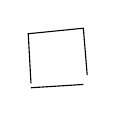
\begin{tikzpicture}[scale=.7]\draw (0,0)--(-.05,.9)--(.95,1)--(1.02,.15);\draw (0,-.08)--(.95,-.02);\end{tikzpicture}}

\uuline{Donc} en résumé

\uline{Proposition} Soit une courbe elliptique \deleted{réelle} complexe. \inserted{$X$}
\deleted{Pour qu'elle admette des}\inserted{Les} structures réelles \deleted{\unsure{sur}\unsure{ elle}}.
\deleted{qu'elles} correspondent aux \inserted{anti} autos \deleted{involutifs} de la
courbe \inserted{elliptique} conforme \deleted{\unsure{fournis}\unsure{ qu'il y en a}},\inserted{il y en a} si et seulement
si la suite
\diagram{\begin{tikzcd}[ampersand replacement=\&]
\unsure{0|1}\arrow[r,dash]\&G^+\arrow[r,dash]\&G\arrow[r,dash]\&\pm1\arrow[r,dash]\&\unsure{0|1}
\end{tikzcd}}
est exacte (à droite). Dans ce cas, $G$ est \deleted{\unsure{un}}\inserted{isom. au} groupe diédral
\inserted{$D_n$} dont $G^+$ (d'ordre $n=2,4$ ou $6$) est le groupe des rotations.
L'ens des structures réelles se partage en deux
orbites sous $G^+$ (opérant par autos intérieurs), et
les structures réelles correspondant à deux orbites
distinctes sont (par définition !) non isomorphes. \deleted{\unsure{et les}
deux orbites correspondent aux structures $E_a,E'_a$}

Je présume que si l'une est formée de structures
$E_a$ ($a\in\mathbb R^{*+}$ fixé), l'autre est formée des structures $E'_{\unsure{a|b}}$
(avec $b\unsure{=|\ne}a$), et inversement, i.e. qu'on peut trouver
un $a\in\mathbb R^{*+}$ unique, tel que les deux orbites sont
l'une formée de structures isom. à $E_a$, l'autre de
structures isom. à $E'_a$. De plus il faudrait

\scanpage{96}
% archive foliation: 98
\begin{verbatim}
//*   FATAR   0338        I
        00000000      00000000      00000000     2222222222
      0000000000    0000000000    0000000000   222222222222
    00      0000  00      0000  00      0000  22        22
   00     00 00  00     00 00  00     00 00           22
  00     00 00  00     00 00  00     00 00           22
 00     00 00  00   00   00  00   00   00          22
00  00    00  00  00    00  00  00    00         22
00 00     00  00 00    00  00 00     00        22
0000      00  0000     00  0000      00     22
000       00  000      00  000       00   22
0000000000    0000000000    0000000000   222222222222
00000000      00000000      00000000   222222222222

\end{verbatim}
\begin{tabular}{@{}l@{}}
\unsure{\texttt{FFFFFFFFFFFF~~~~AAAAAAAAAA~~~TTTTTTTTTTTT~~~~AAAAAAAAAA~~~RRRRRRRRRRR}}\\
\unsure{\texttt{FFFFFFFFFFFF~~~AAAAAAAAAAAA~~TTTTTTTTTTTT~~~AAAAAAAAAAAA~~RRRRRRRRRRRR}}\\
\unsure{\texttt{FF~~~~~~~~~~~~~AA~~~~~~~~AA~~~~~~TT~~~~~~~AA~~~~~~~~AA~~RR~~~~~~~~RR}}\\
\unsure{\texttt{FF~~~~~~~~~~~~~AA~~~~~~~~AA~~~~~~TT~~~~~~~AA~~~~~~~~AA~~RR~~~~~~~~RR}}\\
\unsure{\texttt{FF~~~~~~~~~~~~~AA~~~~~~~~AA~~~~~~TT~~~~~~~AA~~~~~~~~AA~~RR~~~~~~~~RR}}\\
\unsure{\texttt{FFFFFFFF~~~~~~~AAAAAAAAAAAA~~~~~~TT~~~~~~~AAAAAAAAAAAA~~RRRRRRRRRRRR}}\\
\unsure{\texttt{FFFFFFFF~~~~~~~AAAAAAAAAAAA~~~~~~TT~~~~~~~AAAAAAAAAAAA~~RRRRRRRRRRR}}\\
\unsure{\texttt{FF~~~~~~~~~~~~~AA~~~~~~~~AA~~~~~~TT~~~~~~~AA~~~~~~~~AA~~RR~~~~RR}}\\
\unsure{\texttt{FF~~~~~~~~~~~~~AA~~~~~~~~AA~~~~~~TT~~~~~~~AA~~~~~~~~AA~~RR~~~~~RR}}\\
\unsure{\texttt{FF~~~~~~~~~~~~~AA~~~~~~~~AA~~~~~~TT~~~~~~~AA~~~~~~~~AA~~RR~~~~~~RR}}\\
\unsure{\texttt{FF~~~~~~~~~~~~~AA~~~~~~~~AA~~~~~~TT~~~~~~~AA~~~~~~~~AA~~RR~~~~~~~RR}}\\
\unsure{\texttt{FF~~~~~~~~~~~~~AA~~~~~~~~AA~~~~~~TT~~~~~~~AA~~~~~~~~AA~~RR~~~~~~~~RR}}\\
\end{tabular}

\figure{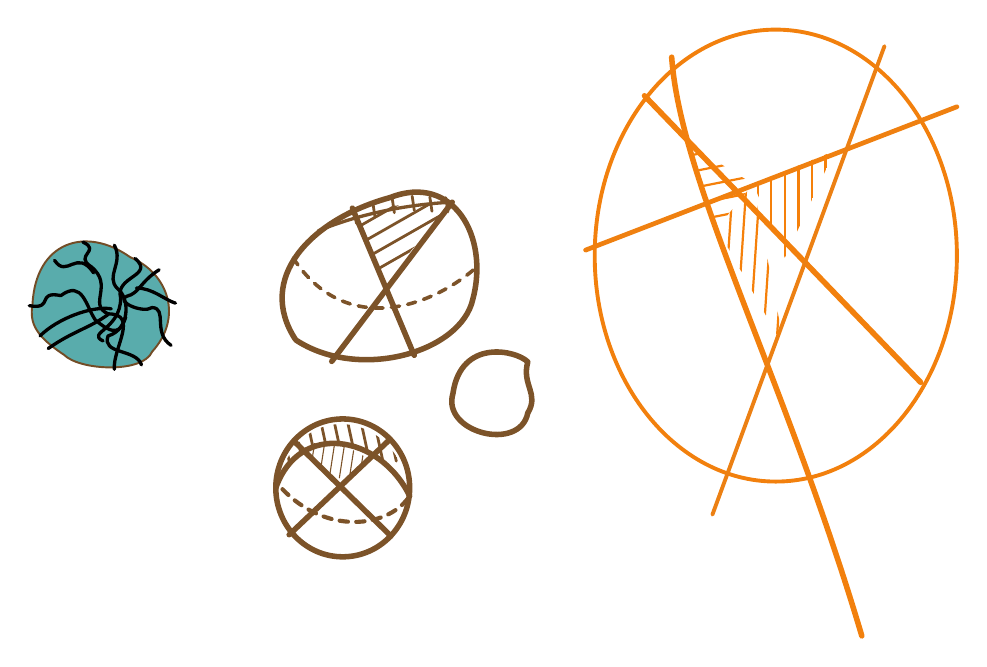
\begin{tikzpicture}[x=1cm,y=1cm,line cap=round,line join=round]
\begin{scope}[shift={(1.5,3.3)},scale=.8]
\filldraw[fill=teal!65,draw=brown!60!black,line width=.7pt] (-1.05,.1) .. controls(-1,1.1) and(-.2,1.35)..(.5,.85) .. controls(1.1,.6) and(1.35,-.1)..(.85,-.65) .. controls(.7,-1.0) and(-.3,-.95)..(-.55,-.7) .. controls(-1.0,-.4) and(-1.1,-.2)..cycle;
\draw[very thick](-.25,1.09)..controls(.05,.95)and(-.4,.88)..(-.12,.7)..controls(.25,.4)and(-.18,.1)..(.15,-.05)..controls(.65,-.05)and(.22,-.6)..(.25,-.93);
\draw[very thick](-.7,.8)..controls(-.5,.5)and(-.35,1.0)..(-.08,.6);
\draw[very thick](.25,1.04)..controls(.4,.75)and(.1,.55)..(.3,.35)..controls(.5,.2)and(.5,-.3)..(.15,-.4)..controls(.04,-.7)and(.6,-.6)..(.68,-.86);
\draw[very thick](.58,.83)..controls(.9,.55)and(.25,.55)..(.35,.2)..controls(.35,-.3)and(-.2,-.35)..(.07,-.48);
\draw[very thick](.96,.65)..controls(.65,.45)and(.65,.28)..(.45,.23)..controls(.25,.15)and(.7,-.05)..(.85,.05)..controls(1.1,.04)and(.85,-.35)..(1.15,-.55);
\draw[very thick](-1.1,.08)..controls(-.7,.01)and(-1,.32)..(-.6,.24)..controls(-.25,.5)and(-.2,.06)..(-.05,-.15)..controls(.25,-.4)and(.35,-.35)..(.43,-.1);
\draw[very thick](-.93,-.4)..controls(-.65,-.12)and(-.1,.08)..(.2,.03);
\draw[very thick](-.8,-.6)..controls(-.4,-.32)and(-.15,-.28)..(.15,-.06);
\draw[very thick](.6,.36)..controls(.86,.36)and(1.05,.17)..(1.22,.12);
\end{scope}
\begin{scope}[shift={(5.1,3.6)},rotate=18]
\draw[brown!65!black,line width=2pt](-1.25,-.3)..controls(-1.5,.6)and(-.6,1.1)..(.45,1.05)..controls(1.3,1.1)and(1.5,.2)..(1.05,-.5)..controls(.7,-1.1)and(-.65,-1.05)..cycle;
\draw[brown!65!black,line width=2pt](-.9,-.7)--(1.18,.75);
\draw[brown!65!black,line width=2pt](-.05,1.07)--(.12,-.95);
\draw[brown!65!black,line width=1.2pt](-.55,.93)..controls(.1,.98)and(.75,.87)..(1.18,.75);
\draw[brown!65!black,line width=1.3pt,dashed](-.96,.7)..controls(-.65,-.45)and(.48,-.45)..(1.22,-.13);
\begin{scope}\clip(-.05,1.07)--(.03,.04)--(1.18,.75)--cycle;\foreach \h in {-.4,-.2,0,.2,.4,.6,.8,1,1.2}{\draw[brown!65!black,line width=1pt](-.15,\h)--(1.3,\h+.3);}\end{scope}
\foreach \x/\y in {-.03/1.05,.22/1.06,.47/1.03,.72/.98,.93/.9,1.12/.83}{\draw[brown!65!black,line width=1pt](\x,\y)--(\x-.03,\y-.18);}
\end{scope}
\begin{scope}[shift={(6.55,2.15)}]
\draw[brown!65!black,line width=2pt](.4,.5)..controls(.25,.65)and(-.45,.8)..(-.55,.1)..controls(-.7,-.4)and(.3,-.65)..(.4,-.15)..controls(.55,.1)and(.32,.2)..(.4,.5);
\end{scope}
\begin{scope}[shift={(4.6,1.05)},scale=.85]
\draw[brown!65!black,line width=2pt](0,0)ellipse(1 and 1.03);
\draw[brown!65!black,line width=2pt](-.8,-.7)--(.7,.72);\draw[brown!65!black,line width=2pt](-.73,.7)--(.72,-.72);
\draw[brown!65!black,line width=2pt](-1,0)..controls(-.65,1)and(.55,.8)..(1,-.12);
\draw[brown!65!black,line width=1.5pt,dashed](-.9,-.02)..controls(-.25,-.7)and(.65,-.6)..(.98,-.15);
\begin{scope}\clip(-.98,.03)..controls(-.65,1)and(.55,.8)..(.99,-.12)..controls(.9,1.1)and(-.65,1.45)..cycle;\foreach \h in {-.8,-.6,-.4,-.2,0,.2,.4,.6,.8}{\draw[brown!65!black,line width=1pt](\h,.4)--(\h-.13,1.0);}\end{scope}
\begin{scope}\clip(-.65,.64)--(0,0)--(.4,.42)..controls(0,.7)and(-.3,.7)..cycle;\foreach\h in {-.5,-.35,-.2,-.05,.1,.25}{\draw[brown!65!black](\h,.15)--(\h+.1,.8);}\end{scope}
\end{scope}
\begin{scope}[shift={(10.1,4)},xscale=1.15,yscale=1.4]
\draw[orange!80!brown,line width=1.4pt](0,0)ellipse(2.0 and 2.05);
\draw[orange!80!brown,line width=2pt](-1.45,1.45)--(1.6,-1.15);
\draw[orange!80!brown,line width=2pt](-1.15,1.8)..controls(-1.05,.65)and(.1,-1.1)..(.95,-3.45);
\draw[orange!75!brown,line width=1.7pt](-2.1,.05)--(2.0,1.35);
\draw[orange!70!brown,line width=1.4pt](1.2,1.9)--(-.7,-2.35);
\begin{scope}\clip(-.94,1.0)--(-.65,.25)--(-.25,.65)--cycle;\foreach\h in {.3,.45,.6,.75,.9}{\draw[orange!85!brown,thick](-1,\h)--(-.2,\h+.13);}\end{scope}
\begin{scope}\clip(-.65,.25)--(.1,-.85)--(-.25,.65)--cycle;\foreach\h in {-.6,-.45,-.3,-.15,0,.15}{\draw[orange!85!brown,thick](\h,-.9)--(\h+.13,.7);}\end{scope}
\begin{scope}\clip(-.25,.65)--(.1,-.02)--(.65,.95)--cycle;\foreach\h in {-.2,-.05,.1,.25,.4,.55}{\draw[orange!85!brown,thick](\h,-.1)--(\h,.95);}\end{scope}
\end{scope}
\end{tikzpicture}}
% crop-candidate: scan 96
\begin{verbatim}
****A  END  JOB  338  FATAR       ROOM     3.01.58 PM 19 AUG 82  R6.PR1  SYS JES2  JOB 338  END  A****
****A  END  JOB  338  FATAR       ROOM     3.01.58 PM 19 AUG 82  R6.PR1  SYS JES2  JOB 338  END  A****
****A  END  JOB  338  FATAR       ROOM     3.01.58 PM 19 AUG 82  R6.PR1  SYS JES2  JOB 338  END  A****
****A  END  JOB  338  FATAR       ROOM     3.01.58 PM 19 AUG 82  R6.PR1  SYS JES2  JOB 338  END  A****
****A  END  JOB  338  FATAR       ROOM     3.01.58 PM 19 AUG 82  R6.PR1  SYS JES2  JOB 338  END  A****
****A  END  JOB  338  FATAR       ROOM     3.01.58 PM 19 AUG 82  R6.PR1  SYS JES2  JOB 338  END  A****
\end{verbatim}
\figure{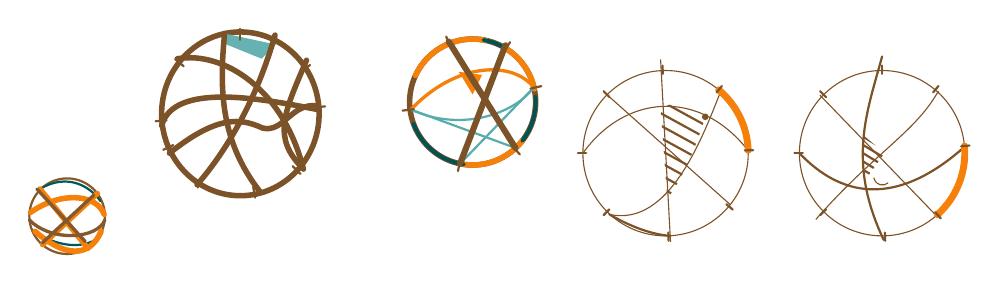
\begin{tikzpicture}[line cap=round,line join=round]
\begin{scope}[shift={(.5,.2)},scale=.48]
\draw[brown!70!black,thick](0,0)circle(1);
\draw[teal!70!black,thick](-.72,.72)..controls(0,1.15)and(.6,.8)..(.88,.4);\draw[teal!70!black,thick](-.9,-.4)..controls(-.1,-.9)and(.5,-.8)..(.78,-.6);
\draw[orange!85!brown,line width=2pt](-.72,.72)--(.55,-.85);\draw[orange!85!brown,line width=2pt](-.65,-.75)--(.8,.6);
\draw[orange!85!brown,line width=2pt](-.97,.1)..controls(-.1,.7)and(.8,.55)..(.98,.05);
\draw[orange!85!brown,line width=2pt](-.85,-.4)..controls(-.05,-1.1)and(.6,-1.1)..(.9,-.4);
\draw[brown!70!black,very thick](-.8,.72)--(.48,-.67);\draw[brown!70!black,very thick](-.65,-.7)--(.7,.55);\draw[brown!70!black,very thick](-1,-.1)..controls(-.4,-.7)and(.8,-.6)..(1,-.1);
\end{scope}
\begin{scope}[shift={(2.7,1.5)}]
\draw[brown!65!black,line width=2pt](0,0)ellipse(1 and 1.04);
\fill[teal!60](-.2,1.02)--(.45,.88)--(.27,.7)--(-.2,.89)--cycle;
\draw[brown!65!black,line width=2pt](-.2,1.02)..controls(-.27,.3)and(-.25,-.35)..(.25,-.99);
\draw[brown!65!black,line width=2pt](.44,1.0)..controls(.2,.15)and(-.2,-.5)..(-.55,-.9);
\draw[brown!65!black,line width=2pt](.84,.68)..controls(.55,.0)and(.4,-.3)..(.8,-.7);
\draw[brown!65!black,line width=2pt](-.8,.7)..controls(-.2,.8)and(.55,.3)..(.8,-.7);
\draw[brown!65!black,line width=2pt](-1,-.15)..controls(-.85,.4)and(.25,.2)..(1,.05);
\draw[brown!65!black,line width=2pt](-.9,-.5)..controls(-.3,-.02)and(.0,-.05)..(.28,-.18)..controls(.55,-.25)and(.65,.15)..(.98,.1);
\foreach\a in {90,65,35,5,-45,-80,-120,-155,185,140}{\draw[brown!65!black,thick](\a:.94)--(\a:1.08);}
\end{scope}
\begin{scope}[shift={(5.65,1.65)},scale=.8]
\draw[brown!65!black,line width=2pt](0,0)circle(1);
\draw[orange!85!brown,line width=2pt](155:1)arc(155:78:1);\draw[orange!85!brown,line width=2pt](60:1)arc(60:12:1);\draw[orange!85!brown,line width=2pt](-38:1)arc(-38:-98:1);
\draw[teal!65!black,line width=1.4pt](80:1)arc(80:62:1);\draw[teal!65!black,line width=1.4pt](5:1)arc(5:-38:1);\draw[teal!65!black,line width=1.4pt](-98:1)arc(-98:-160:1);
\draw[orange!85!brown,very thick](-.98,-.12)..controls(-.25,.65)and(.65,.65)..(.97,.23);
\draw[teal!65,thick](-.98,-.12)..controls(-.2,-.48)and(.65,-.2)..(.97,.23);
\draw[teal!65,thick](-.98,-.12)--(.68,-.73);\draw[teal!65,thick](-.2,-.98)--(.97,.23);
\fill[orange!85!brown](-.22,.48)--(.15,.43)--(.0,.12)--cycle;
\draw[brown!65!black,line width=2.2pt](-.38,.96)--(.68,-.73);\draw[brown!65!black,line width=2.2pt](.52,.9)--(-.2,-.98);
\foreach\a in {112,58,13,-48,-102,187}{\draw[brown!65!black,thick](\a:.94)--(\a:1.12);}
\end{scope}
\begin{scope}[shift={(8.1,1.0)},scale=1.05]
\draw[brown!65!black,thin](0,0)circle(1);
\draw[brown!65!black](-.7,.7)--(.78,-.62);\draw[brown!65!black](-.06,1.13)--(.06,-1.07);
\draw[brown!65!black](-1,0)..controls(-.5,.7)and(.4,.8)..(1,.03);
\draw[brown!65!black](-.68,-.74)..controls(.05,-.9)and(.45,.2)..(.68,.78);
\draw[brown!65!black,thick](-.68,-.74)..controls(-.35,-.93)and(-.1,-.99)..(.06,-1);
\draw[orange!85!brown,line width=2.5pt](50:1)arc(50:2:1);
\fill[brown!65!black](.48,.44)circle(.04);
\begin{scope}\clip(-.06,.54)..controls(.1,.65)and(.3,.58)..(.48,.44)..controls(.3,-.15)and(.1,-.45)..(.02,-.55)--cycle;\foreach\h in {-.5,-.35,-.2,-.05,.1,.25,.4,.55,.7}{\draw[brown!65!black,thick](-.18,\h+.15)--(.55,\h-.25);}\end{scope}
\foreach\a in {92,135,180,-135,-88,-40,50,2}{\draw[brown!65!black,thick](\a:.96)--(\a:1.06);}
\end{scope}
\begin{scope}[shift={(10.85,1.0)},scale=1.05]
\draw[brown!65!black,thin](0,0)circle(1);
\draw[brown!65!black]( -.75,.7)--(.67,-.77);\draw[brown!65!black](-.8,-.8)..controls(-.1,.0)and(.4,.25)..(.68,.75);
\draw[brown!65!black,thick](0,1.17)..controls(-.18,.5)and(-.43,-.1)..(.02,-1.05);
\draw[brown!65!black,thick](-1,.0)..controls(-.35,-.68)and(.35,-.5)..(1,.08);
\draw[orange!85!brown,line width=2.5pt](5:1)arc(5:-48:1);
\begin{scope}\clip(-.23,.22)--(.03,.0)--(-.21,-.33)--cycle;\foreach\h in {-.25,-.15,-.05,.05,.15}{\draw[brown!65!black,thick](-.28,\h+.08)--(.05,\h-.12);}\end{scope}
\draw[brown!65!black](-.1,-.3)..controls(-.07,-.4)and(.02,-.4)..(.07,-.36);
\foreach\a in {90,135,180,-135,-88,-48,50,5}{\draw[brown!65!black,thick](\a:.96)--(\a:1.06);}
\end{scope}
\end{tikzpicture}}

\scanpage{97}
% archive foliation: 99
expliciter le lien du paramètre $a$ avec le paramètre $\tau$, ou
mieux, avec l'invariant modulaire $j\in\mathbb R^{\unsure{2|*}}$ (serait-ce
$j=\unsure{\tfrac14|4}\log a$ ?)
\deleted{\inserted{\unsure{i.e.} $a=\exp j$ ou $a=\exp(-j)$}\unsure{suivant qu'on est dans la famille} $E_a,E'_a$ ?}.

\deleted{Considérons} Notons que si $\sigma$ est dans $G^-$, alors
suivant les cas $-\sigma$ est conjugué, ou non conjugué,
à $\sigma$. \inserted{(réflexion p.r. à la \unsure{droite orthogonale} à celle de $\sigma$)}
Dans le cas hexagonal, il est non conjugué ;
dans le cas carré, il est conjugué. Dans le cas
non \unsure{anharmonique}, $n=2$, il est bien sûr non conjugué (car
$G$ est alors commutatif) -- donc le cas \deleted{hexagonal}\inserted{carré} est
le seul où $-\sigma$ \deleted{\unsure{ne}} soit \deleted{\unsure{pas}} conjugué à $\sigma$.
\deleted{Donc \unsure{si} dans le cas carré par ex., on trouve}
\figure{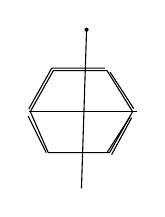
\begin{tikzpicture}[scale=.65]
\draw(-1,0)--(-.55,.8)--(.5,.8)--(1,0)--(.55,-.8)--(-.65,-.8)--cycle;
\draw(-1.03,.05)--(-.58,.85)--(.46,.85);\draw(.56,.77)--(1.02,.06);\draw(-1.04,-.09)--(-.69,-.8);\draw(.95,-.1)--(.5,-.8);\draw(.98,-.12)--(.59,-.84);
\draw(-1.03,0)--(1.08,0);\draw(0,-1.5)--(.1,1.6);\fill(.1,1.6)circle(.04);
\end{tikzpicture}}

\uline{Distinguons les cas}

1) \uline{$n=2$} Cas non \unsure{anharmonique}. Le groupe des autos
est $\pm1,\pm\sigma$, où $\sigma$ est un \inserted{anti} auto. On voit de
suite que si $\sigma$ est du type somme directe d'un
$\operatorname{id}_P$ et $-\operatorname{id}_Q$, il en est de $=$ de $-\sigma$ (avec $P,Q$
échangés) donc on est dans cas $E_a$, \unsure{où}\deleted{\unsure{on}} donc
un $E_a$ et un $E_{a'}$, correspondent aux deux éléments de
$\unsure{\sigma},\sigma'$ de $G^-$, et on aura $aa'=1$.
\deleted{\unsure{En}} car
prenant un gén. $u=\unsure{e_+}$ de $\pi_+$, un autre \inserted{$v=e_-$}$v$ de $\pi_-$, on a
\[
a=a(\sigma)=\frac{Q(\unsure{e_-|e_+})}{Q(e_+)}
\]
et comme par passage de $\sigma$ à $-\sigma$ \deleted{\unsure{les}} $e_+$ et $e_-$ s'interchangent,
on aura bien
\[
a(-\sigma)=1/a(\sigma)
\]
\margin{\figure{\begin{tikzpicture}\draw (0,0)--(0,1.5);\end{tikzpicture}}Ceci vaut aussi bien dans le cas des $E_a$, que des $E'_a$}
(valable dans tous les cas), donc
\[
a(-\sigma)=a(\sigma)\quad\Longleftrightarrow\quad a(\sigma)=1\quad\Longleftrightarrow\quad\text{cas \uline{carré}}.
\]

\scanpage{98}
% archive foliation: 100
2) \uline{Cas carré} $n=4$. On voit que l'on a un $\sigma$ de type $E_1$,
et $-\sigma$ est du $=$ type. Cela correspond aux
symétries p.r. aux \deleted{\unsure{bissectrices}}\inserted{diagonales} du carré de
départ. La symétrie par rapport à un côté
échange $e_0$ et $e_1$, les invariants et anti-invariants
sont resp. engendrés par $e_0+e_1$ et $e_0-e_1$, qui n'engendrent
pas le réseau, donc on est dans le cas $E'_{\unsure{a'}}$. Or
\figure{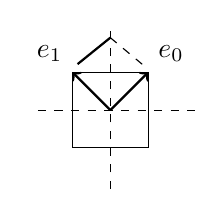
\begin{tikzpicture}[scale=.8]
\draw(-.6,-.6)--(-.6,.6)--(.6,.6)--(.6,-.6)--cycle;
\draw[dashed](-1.15,0)--(1.35,0);\draw[dashed](0,-1.25)--(0,1.3);
\draw[->,thick](0,0)--(-.6,.6)node[above left]{$e_1$};\draw[->,thick](0,0)--(.6,.6)node[above right]{$e_0$};
\draw[thick](-.52,.73)--(0,1.15);\draw[dashed](0,1.15)--(.6,.65);
\end{tikzpicture}}
\[
a'=\frac{Q(e_0-e_1)}{Q(e_0+e_1)}=\deleted{4}1\qquad\text{aussi}
\]
\deleted{$\unsure{E_1}$}
Donc on trouve les types $E_1$ (``sommets'') et $E'_1$ (``côtés'').

3) \uline{Cas hexagonal} $n=6$.

\uline{Réflexions-sommets}. Les \deleted{\unsure{premiers}} invariants pour
la réflexion p.r. à $\mathbb R u$ sont \uline{engendrés}
par $u$, les anti-invariants par $2v-u$, c'est
du type $E'_a$, avec
\figure{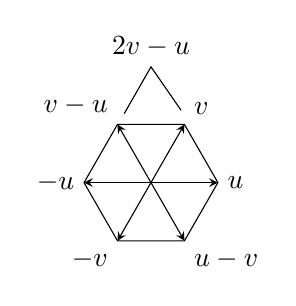
\begin{tikzpicture}[scale=.85,>=stealth]
\draw(-1,0)--(-.5,.87)--(.5,.87)--(1,0)--(.5,-.87)--(-.5,-.87)--cycle;
\draw(-.4,1.03)--(0,1.73)--(.45,1.08);\node[above]at(0,1.73){$2v-u$};
\draw[->](0,0)--(1,0)node[right]{$u$};\draw[->](0,0)--(.5,.87)node[above right]{$v$};
\draw[->](0,0)--(-.5,.87)node[above left]{$v-u$};\draw[->](0,0)--(-1,0)node[left]{$-u$};
\draw[->](0,0)--(-.5,-.87)node[below left]{$-v$};\draw[->](0,0)--(.5,-.87)node[below right]{$u-v$};
\end{tikzpicture}}
\[
a=\frac{Q(2v-u)}{Q(u)}=\sqrt3
\]

\uline{Réflexions-faces} ce sont les $-\sigma$, on trouve donc $E'_{1/a}=E'_{1/\sqrt3}$.

\uline{En résumé} Dans tous les cas, sauf le cas carré, \deleted{\unsure{tous les}}\inserted{l'ens des}
\deleted{les}\inserted{les types de} structures réelles sur $X$ sont soit \deleted{du type}
$\{E_a,E_{1/a}\}$,
\deleted{\unsure{le cas}} soit $\{E'_a,E'_{1/a}\}$ \inserted{avec $a>1$}
(le cas hexagonal étant dans le
deuxième cas \inserted{avec $a=\sqrt3$}), à l'exclusion bien sûr l'un de l'autre.
Dans le cas carré, l'ens des structures réelles
est $\{E_1,E'_1\}$ i.e. il y a à la fois des structures $E$ et $E'$.
\figure{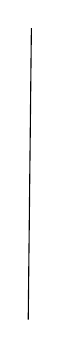
\begin{tikzpicture}\draw(0,0)--(-.04,-3.7);\end{tikzpicture}}

\scanpage{99}
% archive foliation: 101
\uline{Résumé} Cas $E_a$ :
\[
\left\{\begin{array}{l}
\text{base }u=e_0,\ v=e_1\\
\text{forme }\deleted{Q(e_0)=Q(e_1)}\quad Q(xe_0+ye_1)=x^2+ay^2
\end{array}\right.
\]
Si on \unsure{met|veut} la forme $Q$ sous forme standard on
prend la \inserted{nouvelle} base
$\underbrace{e_0}_{1},\underbrace{\frac1{\sqrt a}e_1}_{i}$, on trouve donc la base
$1,\sqrt a\,i$ d'où
\[\boxed{\tau=\sqrt a\,i},\]

Cas $E'_a$ : base, \deleted{$\unsure{u=e_0,v=\frac12u|u=e_0,v=u}$}
distinguée p.r. à $Q$ les
\[
e_0=u,\quad e_1=2v-u;\qquad Q(xe_0+ye_1)=x^2+ay^2
\]
\[v=\frac12(e_0+e_1).\]
\unsure{au|on} \deleted{\unsure{premier}} changement de base.
\[
\underbrace{e_0}_{1},\underbrace{\frac1{\sqrt a}e_1}_{i}
\qquad\text{bien orthonormale}
\]
et on a $u\Rightarrow1$, $v\mapsto\frac12(1+\sqrt a\,i)$, donc
\[\boxed{\tau=\frac12(1+\sqrt a\,i)}=\frac12+\frac{\sqrt a}{2}i.\]
\figure{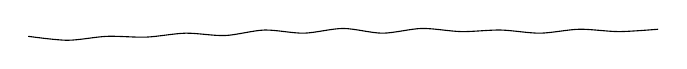
\begin{tikzpicture}\draw plot[smooth]coordinates{(0,0)(.5,-.05)(1,0)(1.5,-.01)(2,.04)(2.5,.01)(3,.08)(3.5,.04)(4,.1)(4.5,.04)(5,.1)(5.5,.06)(6,.08)(6.5,.04)(7,.09)(7.5,.06)(8,.09)};\end{tikzpicture}}

Calcul du groupe des pts réels d'une courbe $E_a$, $E'_a$.

Pts réels sont les $x\bmod\pi$ ($x\in\pi_{\mathbb R}$) tels que
\[\sigma x\equiv x\quad(\pi)\]
\uline{Distinguons les deux cas}.

1) $\uline{E_a}$ \deleted{$\sigma(e_0,e_1)=$} $\sigma(x,y)=x,-y$
\[\text{donc}\qquad\sigma(x,y)-(x,y)=(0,2y)\]
donc la condition est que $2y\in\mathbb Z$. Donc il y a \deleted{\unsure{les}}
les pts de $\deleted{\unsure{\frac02}}\mathbb R e_0$ et de
$\deleted{\mathbb R}(0,\frac12)+\mathbb R e_0$, donc
\uline{deux composantes connexes} \deleted{pour} $X(\mathbb R)$.

\margin{$\unsure{<}$}

\scanpage{100}
% archive foliation: 102
\uline{Cor} Supposons $k$ principal \inserted{$2$-régulier}, $k_0=k/2k$ un corps.
Alors les $(M,\sigma)$ \inserted{\unsure{cat. des}} précédents
\unsure{équiv. à} celles des paires $(P,Q,\deleted{\unsure{\bar p,\bar q,m}})$ où $P,Q$ libres de rg $1$,
et $\deleted{\unsure{p}}m\subset\underbrace{P/2P}_{p}\oplus\underbrace{Q/2Q}_{q}$ un espace vectoriel sur $k_0$,
\deleted{\unsure{de M, qui}}
qui est soit nul, soit une droite $\ne p,q$ (\unsure{droites coordonnées}).

\uline{Cor} Cela donne une description des classes de conjugaison,
d'éléments de $\mathrm{Gl}(2,k)^{\deleted{\unsure{*}}}$ qui sont d'ordre $2$ exactement, et
distincts de $\{\pm1\}$ : il y \deleted{\unsure{en a}} \inserted{celle de}
$\begin{pmatrix}1&0\\0&-1\end{pmatrix}$ (correspondant au
cas $m=0$), puis \uline{une} \deleted{famille, \unsure{indexée} par les \unsure{points de}
$\unsure{\mathbb P|\mathbf P}^1(k_0)$ distincts de $0,\infty$ (en supposant que
$k^\times\to k_0^\times$ est surjectif \unsure{sinon la classification sera plus fine})}
\margin{$\unsure{k'^\times\to k_0'^\times}$ \unsure{surj.}}
\unsure{en fait bien de} $P/2P\unsure{\to}Q/2Q$ en revenant au choix d'une base de $P,Q$.

\unsure{Plus} concrètement :
\[
P=k,\ Q=k,\ m=\text{diagonale de }k_0\oplus k_0\quad\text{i.e.}
\]
\[
M'=(2k\oplus2k)+\text{diag. de }k\oplus k
=\{(x,y)\mid x-y\in2k\}
\]
donc on peut prendre base de $M'$
\[
\unsure{e_0|u}=(2,0),\quad\unsure{e_1|v}=(1,1),\quad
\text{d'où}\quad-\unsure{e_0|u}+2\unsure{e_1|v}=(0,2)=\operatorname{sym}(\unsure{e_0|u})
\]
\margin{\figure{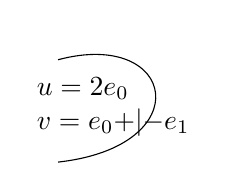
\begin{tikzpicture}\node[align=left] at (0,0) {$u=2e_0$\\$v=e_0\unsure{+|-}e_1$};\draw(-.7,.6)..controls(.8,1)and(1.1,-.5)..(-.7,-.7);\end{tikzpicture}}}
On trouve
\[
\sigma\unsure{e_0|u}=\unsure{e_0|u},\quad
\sigma\unsure{e_1|v}=(1,-1)=e_1-\operatorname{sym}\unsure{e_1|v}=\unsure{e_0-e_1|u-v}
\]
i.e. la matrice de $\sigma$ p.r. à $(\unsure{u,e_1|u,v})$ est
\[\begin{pmatrix}1&1\\0&-1\end{pmatrix}\]

Dans le cas $k=\mathbb Z$, c'est la matrice de la réflexion p.r. la
diagonale $0,e_0$ de l'hexagone régulier,
les \unsure{pts.|fl.} de l'hexagone étant rapportés à un
syst. de coordonnées obliques ayant comme base
deux sommets consécutifs $u$ $v$ ($M$ est le réseau
engendré par \unsure{l'ens|l'un} des sommets).
\figure{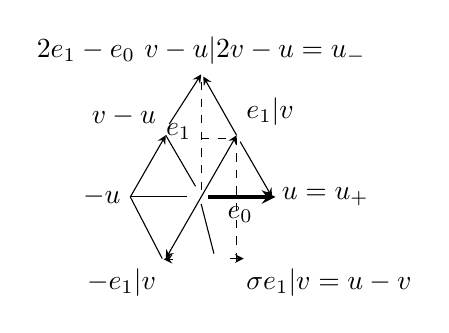
\begin{tikzpicture}[scale=.9,>=stealth]
\draw[->](-1,0)--(-.5,.87);\draw(-.5,.87)--(-.08,.15);
\draw[->](-.45,1.03)--(0,1.73);\draw[->](.5,.87)--(.03,1.7);
\draw[->](.55,.78)--(1,0);\draw[->](.4,-.87)--(.6,-.87);
\draw[->](-.4,-.88)--(-.53,-.88);\draw(-.55,-.87)--(-1,0);
\draw[->](0,0)--(.5,.87);\draw[->](0,0)--(-.5,-.87);
\draw[->,very thick](.1,0)--(1.05,0);\draw(-1,0)--(-.2,0);
\draw[dashed](0,.1)--(0,1.65);\draw[dashed](0,.82)--(.5,.82)--(.5,-.9);
\draw(0,-.1)--(.18,-.8);
\node[left]at(-1,0){$-u$};\node[above left]at(-.5,.87){$v-u$};
\node[above right]at(.5,.87){$\unsure{e_1|v}$};\node[right]at(1,0){$u=u_+$};
\node[below left]at(-.5,-.87){$-\unsure{e_1|v}$};
\node[below right]at(.5,-.87){$\sigma\unsure{e_1|v}=u-v$};
\node[left]at(0,.92){$\unsure{e_1}$};\node[below]at(.55,0){$e_0$};
\node[above]at(0,1.73){$\deleted{\unsure{2e_1-e_0}}\ \unsure{v-u|2v-u}=u_-$};
\end{tikzpicture}}

\uline{NB} Soit $u_+$ une base de $\pi_+$, $u_-$ une base de $\pi_-$, alors
\deleted{dans} On peut représenter $\sigma_{\mathbb R}$ pour la base $(u_+,u_-)$ de $\pi\otimes_{\mathbb Z}\mathbb R$,
par la matrice $\begin{pmatrix}1&0\\0&-1\end{pmatrix}$ le réseau $\pi$ étant identifié
à $\mathbb Z u_-+\mathbb Z u_+$ \deleted{$\unsure{\simeq\mathbb Z^2}$} dans le premier cas et dans le $2$\textsuperscript{d}
à l'ens des $xu_++yu_-$ tels que $x-y\in\mathbb Z$, $x,y\in\frac12\mathbb Z$.
\margin{$\sigma^2(e_1)=\sigma e_0-\sigma e_1=e_0-(e_0-e_1)=e_1$}

\scanpage{101}
% archive foliation: 103
2) $\uline{E'_a}$ Donc $\pi$ engendré par $u,v$ avec $\sigma u=u$, $\sigma v=u-v$
\[\sigma(x,y)=\sigma(xu+yv)=xu+y(u-v)=(x+y)u-yv.\]
\[\sigma(x,y)-(x,y)=yu-2yv=y(u-2v),\quad\text{donc la condition est}\]
$y\in\mathbb Z$, donc on trouve \deleted{que} les points de $\mathbb R\unsure{u_+|u_0}\bmod\pi$,
donc dans ce cas $X(\mathbb R)$ est connexe.

\margin{9.2.}
\uline{NB} Pour bien faire il faudrait aussi classifier les
courbes elliptiques réelles \unsure{intrinsèques}, i.e. les
torseurs (sur $\mathbb R$) sous les \inserted{schémas en} groupes elliptiques
$E_a,E'_a$. Les torseurs non triviaux fournissent les
surfaces conformes \deleted{sans} bord non orientables de
genre $1$. La suite exacte de $\gamma$-modules ($\gamma=\mathrm{Gal}(\mathbb C/\mathbb R)\simeq\{\pm1\}$)
\diagram{\begin{tikzcd}[ampersand replacement=\&]
0\arrow[r]\&\pi\arrow[r]\&V\arrow[r]\&E(\mathbb C)\arrow[r]\&0
\end{tikzcd}}
fournit
\[
H^1(\gamma,E(\mathbb C))\simeq H^2(\gamma,\pi)\simeq
\pi^\gamma/(1+\sigma)\pi=\pi_+/(1+\sigma)\pi
\]
1) Cas de $E_a$. On a $\pi\simeq\pi_+\oplus\pi_-$, d'où $\pi^\gamma=\pi_+$
\[
H^1(\mathbb R,E_{\mathbb R})\simeq H^1(\gamma,E(\mathbb C))\simeq H^2(\gamma,\pi)
\simeq\underset{\substack{\Vert\\\mathbb Z/2\mathbb Z}}{\uline{H^2(\gamma,\pi_+)}}
\oplus\underset{\substack{\Vert\\0}}{\uline{H^2(\gamma,\pi_-)}}
\]
Il y a exactement une classe non
nulle dans $H^1$, qui est d'ordre $2$.

2) Cas de $E'_a$. On a $H^1(\mathbb R,E_{\mathbb R})\simeq0$.

Donc les seules courbes elliptiques vraiment
\unsure{intrinsèques} sur $\mathbb R$ sont les $E_a^!=$ torseurs non
triviaux (d'ordre $2$) sous $E_a$, dépendant du
paramètre $a\in\mathbb R^{*+}$.
